\section{Résolution numérique par la méthode RK4}

\subsection{Formulation pour le système de Lorenz}
La méthode RK4 s'applique au système de Lorenz en traitant simultanément les trois équations couplées. Pour un état $\mathbf{u} = (X, Y, Z)$, le système peut s'écrire sous la forme :

\begin{equation}
\frac{d\mathbf{u}}{dt} = \mathbf{f}(\mathbf{u}) = \begin{pmatrix}
Y - X \\
-\frac{1}{\tau}Y + XZ \\
R - \frac{1}{\tau}Z - XY
\end{pmatrix}
\end{equation}

\subsubsection{Calcul des coefficients}
Les coefficients $k_i$ de la méthode RK4 sont calculés comme suit :

\begin{align}
k_1 &= \mathbf{f}(t_n, \mathbf{u}_n) \\
k_2 &= \mathbf{f}(t_n + \frac{h}{2}, \mathbf{u}_n + \frac{h}{2}k_1) \\
k_3 &= \mathbf{f}(t_n + \frac{h}{2}, \mathbf{u}_n + \frac{h}{2}k_2) \\
k_4 &= \mathbf{f}(t_n + h, \mathbf{u}_n + hk_3)
\end{align}

où $h$ est le pas de temps et $\mathbf{u}_n$ est l'état du système au temps $t_n$.

\subsection{Implémentation}

\subsubsection{Structure du code}
Le solveur RK4 est implémenté comme une sous-routine Fortran qui prend en compte les spécificités du système de Lorenz :

\begin{lstlisting}[language=Fortran,caption=Implémentation RK4 pour le système de Lorenz]
module rk4_solver
    use types, only: dp
    implicit none

    type :: LorenzState
        real(dp) :: X, Y, Z
    end type LorenzState

contains
    subroutine solve_step(state, dt, tau, R)
        type(LorenzState), intent(inout) :: state
        real(dp), intent(in) :: dt, tau, R
        type(LorenzState) :: k1, k2, k3, k4, temp
        
        ! Calcul de k1
        k1%X = state%Y - state%X
        k1%Y = -state%Y/tau + state%X * state%Z
        k1%Z = R - state%Z/tau - state%X * state%Y
        
        ! Calcul de k2
        temp = state
        temp%X = state%X + dt*k1%X/2
        temp%Y = state%Y + dt*k1%Y/2
        temp%Z = state%Z + dt*k1%Z/2
        k2%X = temp%Y - temp%X
        k2%Y = -temp%Y/tau + temp%X * temp%Z
        k2%Z = R - temp%Z/tau - temp%X * temp%Y
        
        ! Calcul de k3
        temp%X = state%X + dt*k2%X/2
        temp%Y = state%Y + dt*k2%Y/2
        temp%Z = state%Z + dt*k2%Z/2
        k3%X = temp%Y - temp%X
        k3%Y = -temp%Y/tau + temp%X * temp%Z
        k3%Z = R - temp%Z/tau - temp%X * temp%Y
        
        ! Calcul de k4
        temp%X = state%X + dt*k3%X
        temp%Y = state%Y + dt*k3%Y
        temp%Z = state%Z + dt*k3%Z
        k4%X = temp%Y - temp%X
        k4%Y = -temp%Y/tau + temp%X * temp%Z
        k4%Z = R - temp%Z/tau - temp%X * temp%Y
        
        ! Mise à jour finale
        state%X = state%X + (dt/6)*(k1%X + 2*k2%X + 2*k3%X + k4%X)
        state%Y = state%Y + (dt/6)*(k1%Y + 2*k2%Y + 2*k3%Y + k4%Y)
        state%Z = state%Z + (dt/6)*(k1%Z + 2*k2%Z + 2*k3%Z + k4%Z)
    end subroutine solve_step
end module rk4_solver
\end{lstlisting}

\subsection{Analyse des résultats}


\subsubsection{Paramètres de simulation}
Les simulations ont été réalisées avec les paramètres suivants :

\begin{itemize}
    \item \textbf{Pas de temps} : $h = 0.01$
    \item \textbf{Durée totale} : $T = 100.0$
    \item \textbf{Amplitude des ondes} : $R = 2.5$
    \item \textbf{Conditions initiales} : $(X_0, Y_0, Z_0) = (1.0, 0.0, 0.0)$
\end{itemize}


% \subsubsection{Caractéristiques des différents régimes}
% \begin{itemize}
%     \item $\tau$ = 0.5 : Amortissement rapide des oscillations (État Non-Marcheur)
%     \item $\tau$ = 2.0 : Établissement d'états stationnaires symétriques (Marche Régulière)
%     \item $\tau$ = 5.0 : Oscillations périodiques avec motifs complexes (Marche Chaotique)
%     \item $\tau$ = 8.9 : Dynamique chaotique avec attracteur étrange (Oscillations avec Dérive)
% \end{itemize}


% \subsection{Analyse des régimes dynamiques}
En fonction du paramètre de mémoire $\tau$, le système présente différents comportements caractéristiques.

\subsubsection{État Non-Marcheur ($\tau$ = 0.5) }
Pour une faible valeur de $\tau$, le système converge rapidement vers un point fixe.

On peut également noter que la trajectoire converge rapidement vers l'origine (X → 0) et l'absence d'oscillations.

\begin{figure}[H]
    \centering
    \begin{subfigure}[b]{0.5\textwidth}
        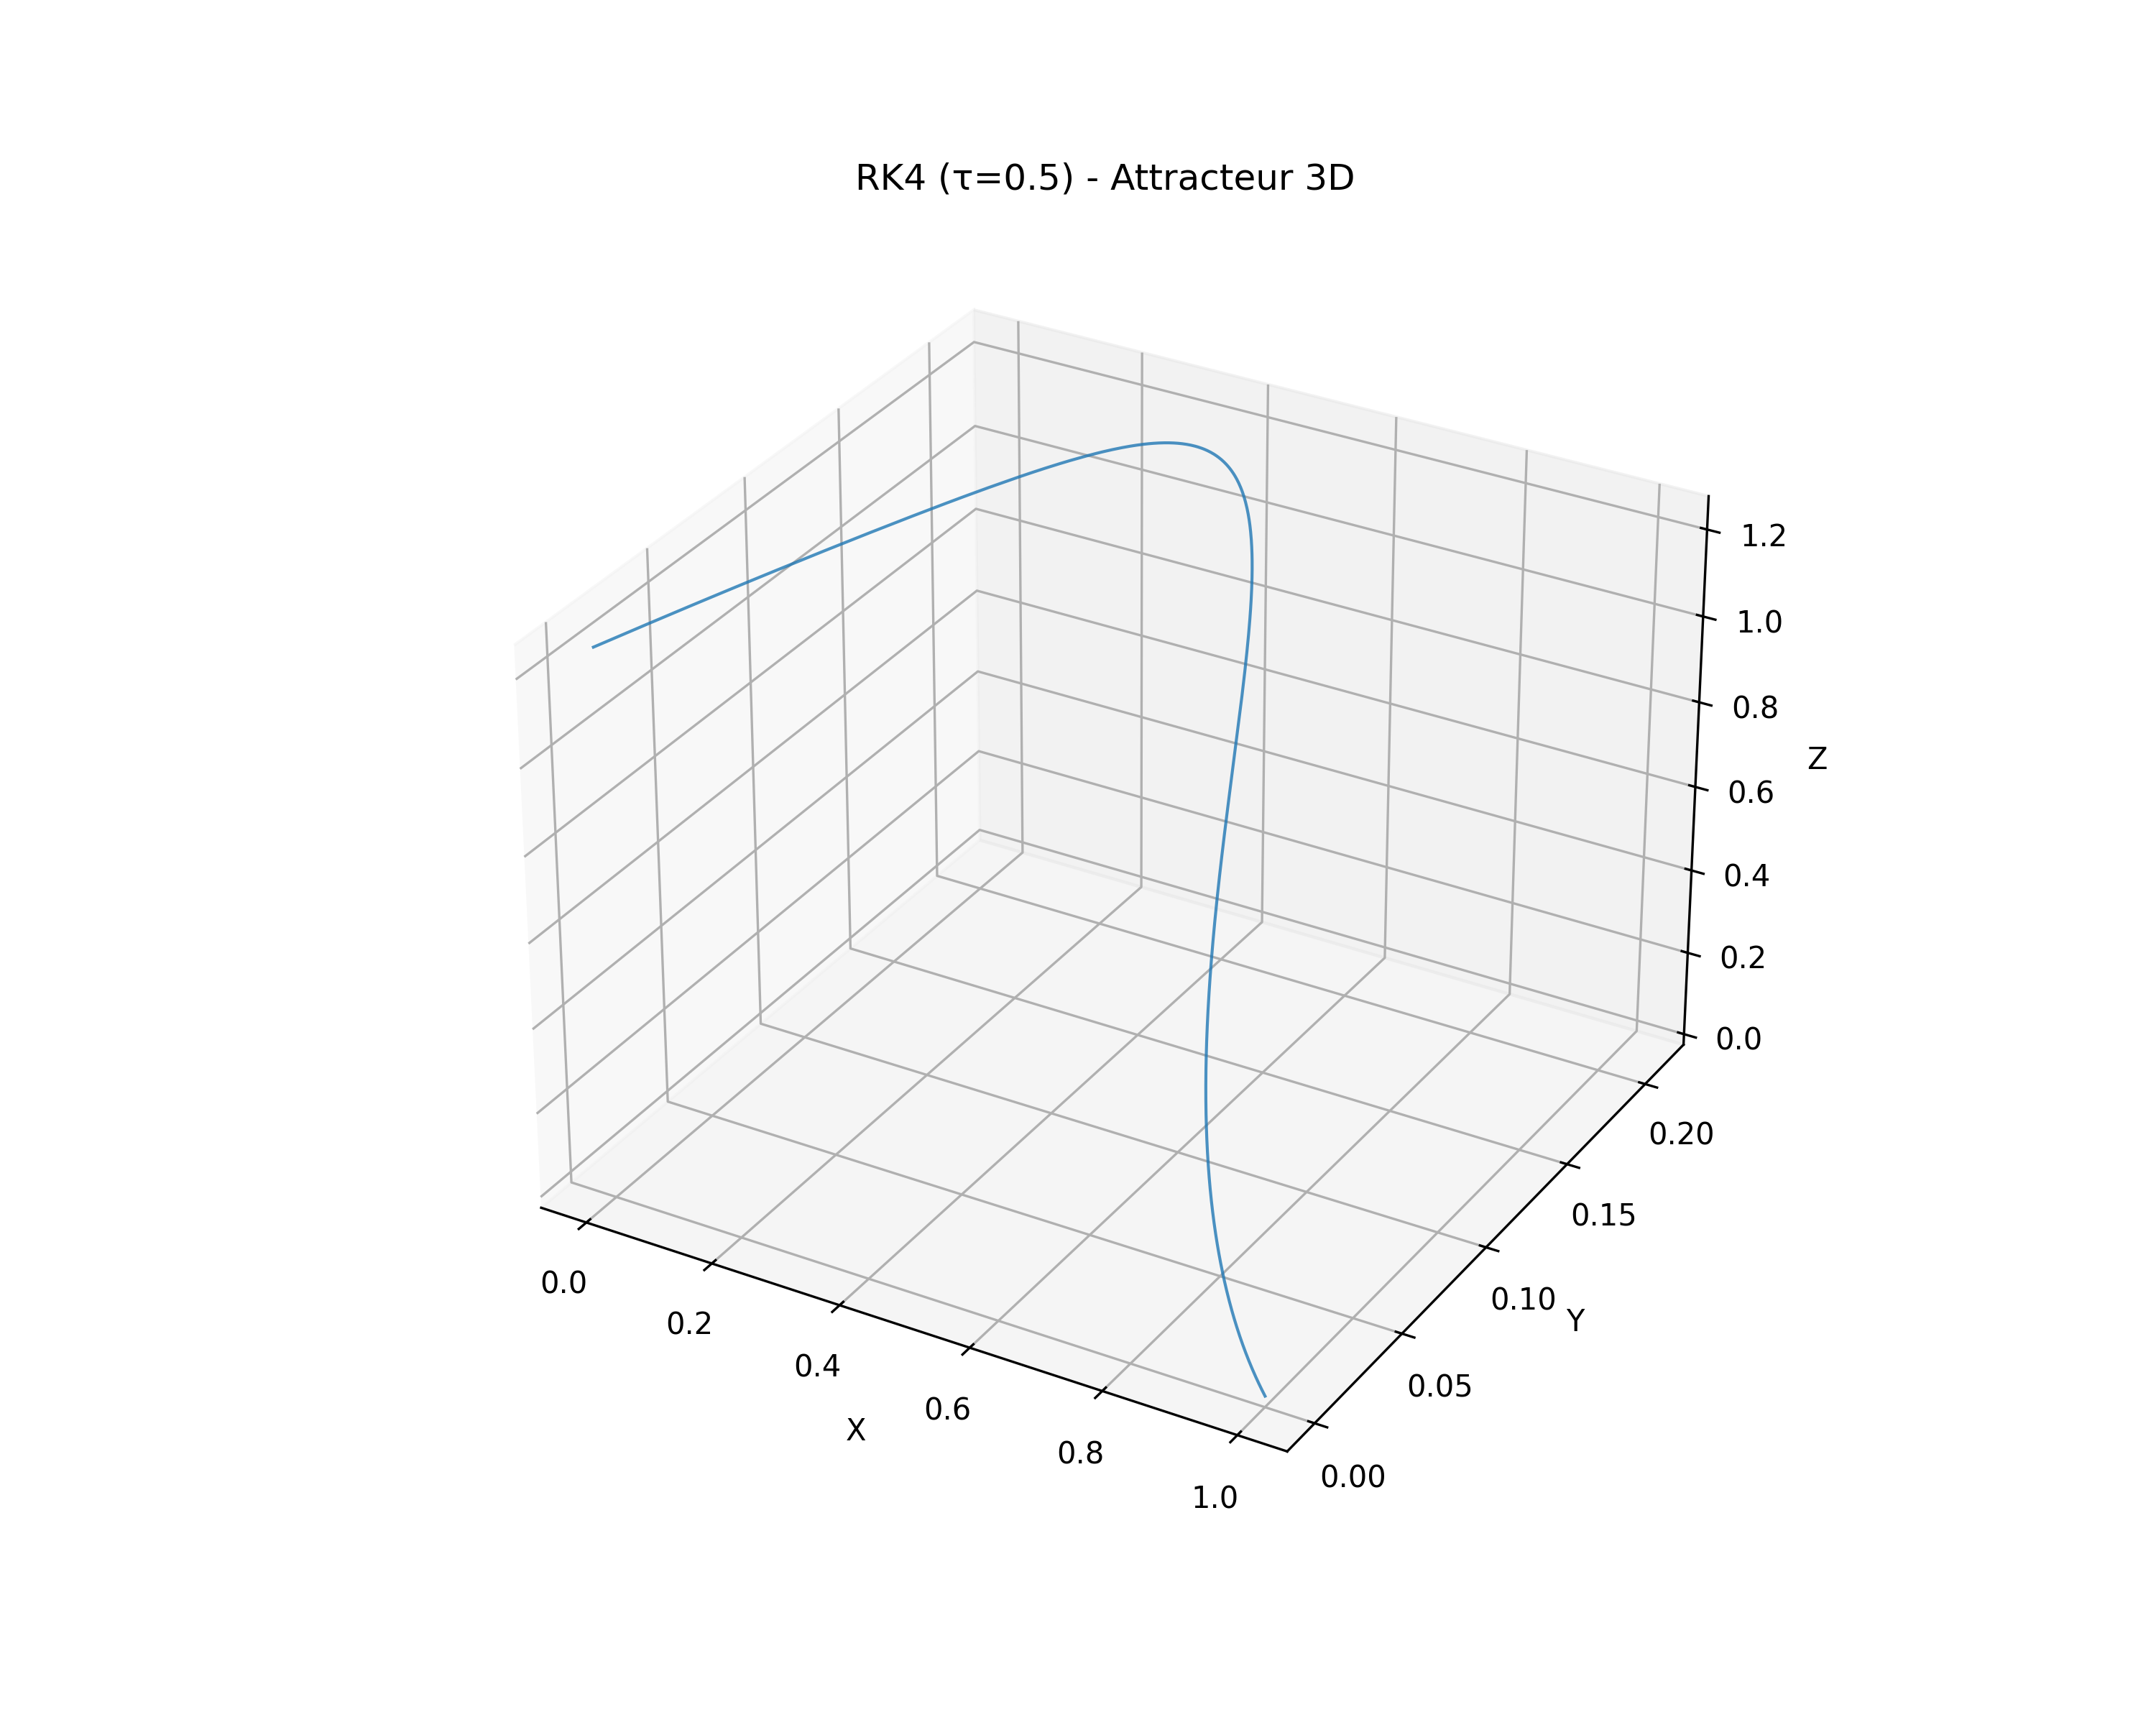
\includegraphics[width=\textwidth]{figures/rk4/rk4_tau0.5_3d}
        \caption{Trajectoire 3D}
    \end{subfigure}
    \begin{subfigure}[b]{0.4\textwidth}
        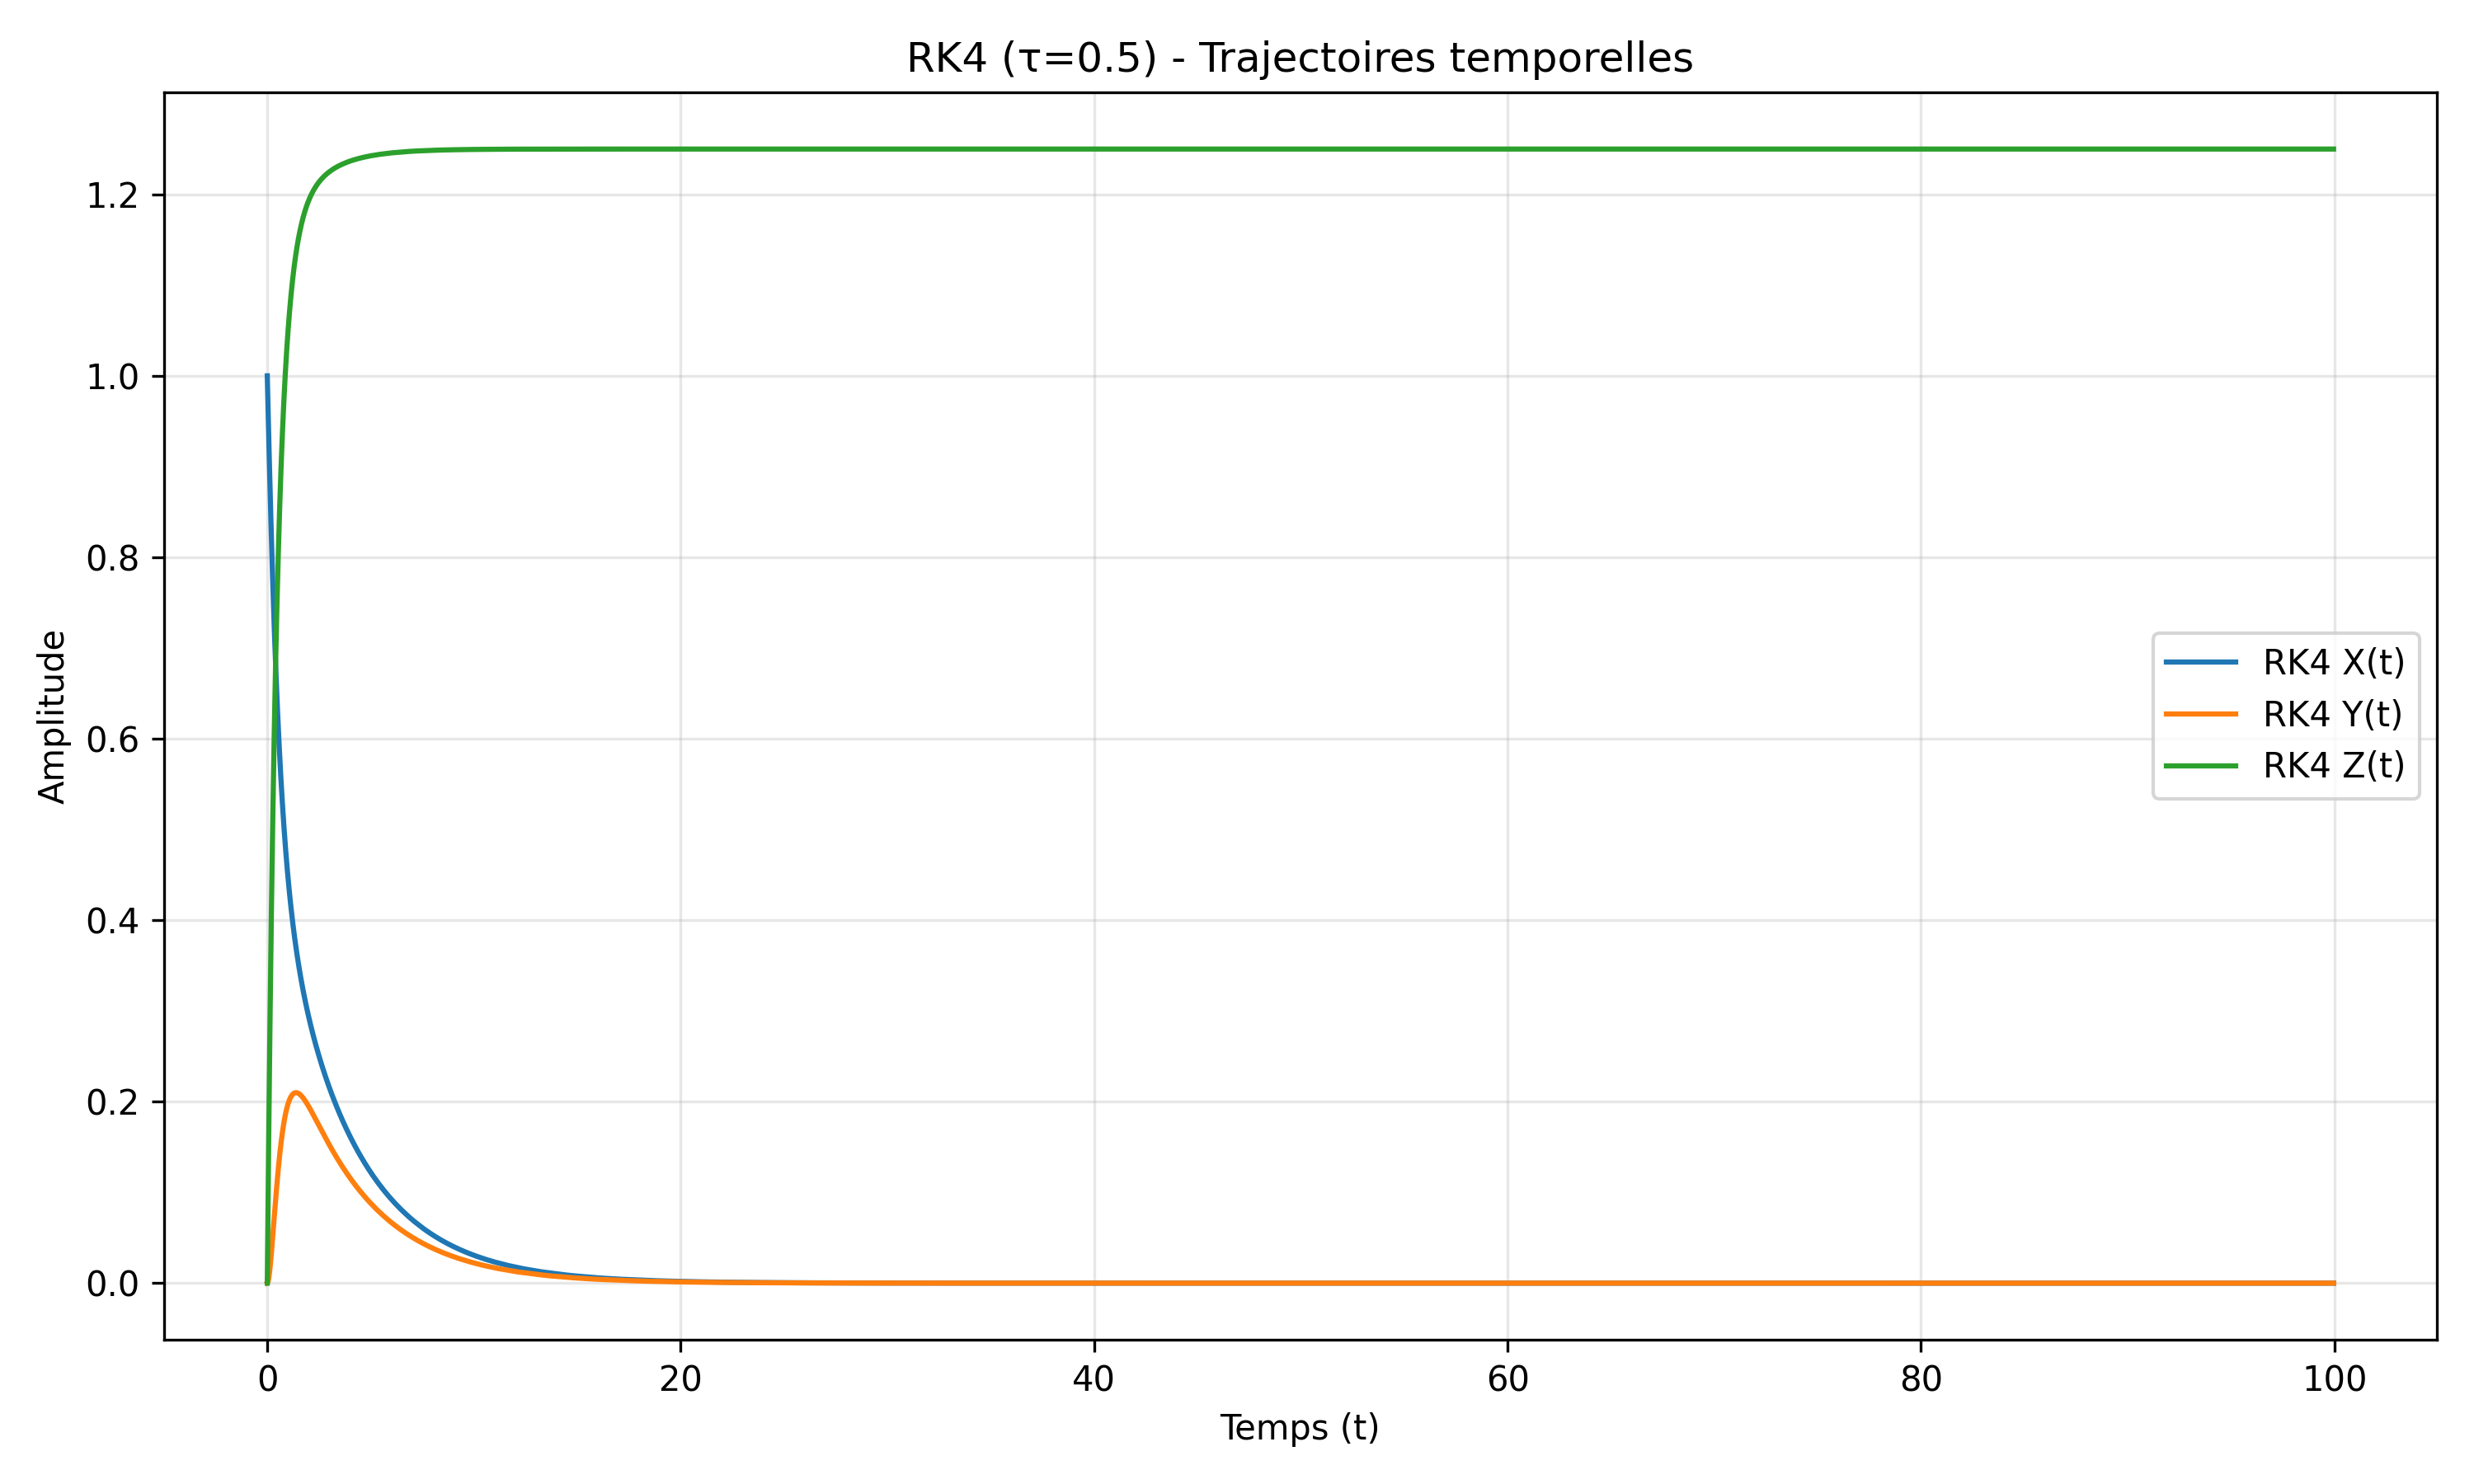
\includegraphics[width=\textwidth]{figures/rk4/rk4_tau0.5_time}
        \caption{Évolution temporelle : X converge rapidement vers zéro, Y et Z se stabilisent}
    \end{subfigure}
    \begin{subfigure}[b]{0.3\textwidth}
        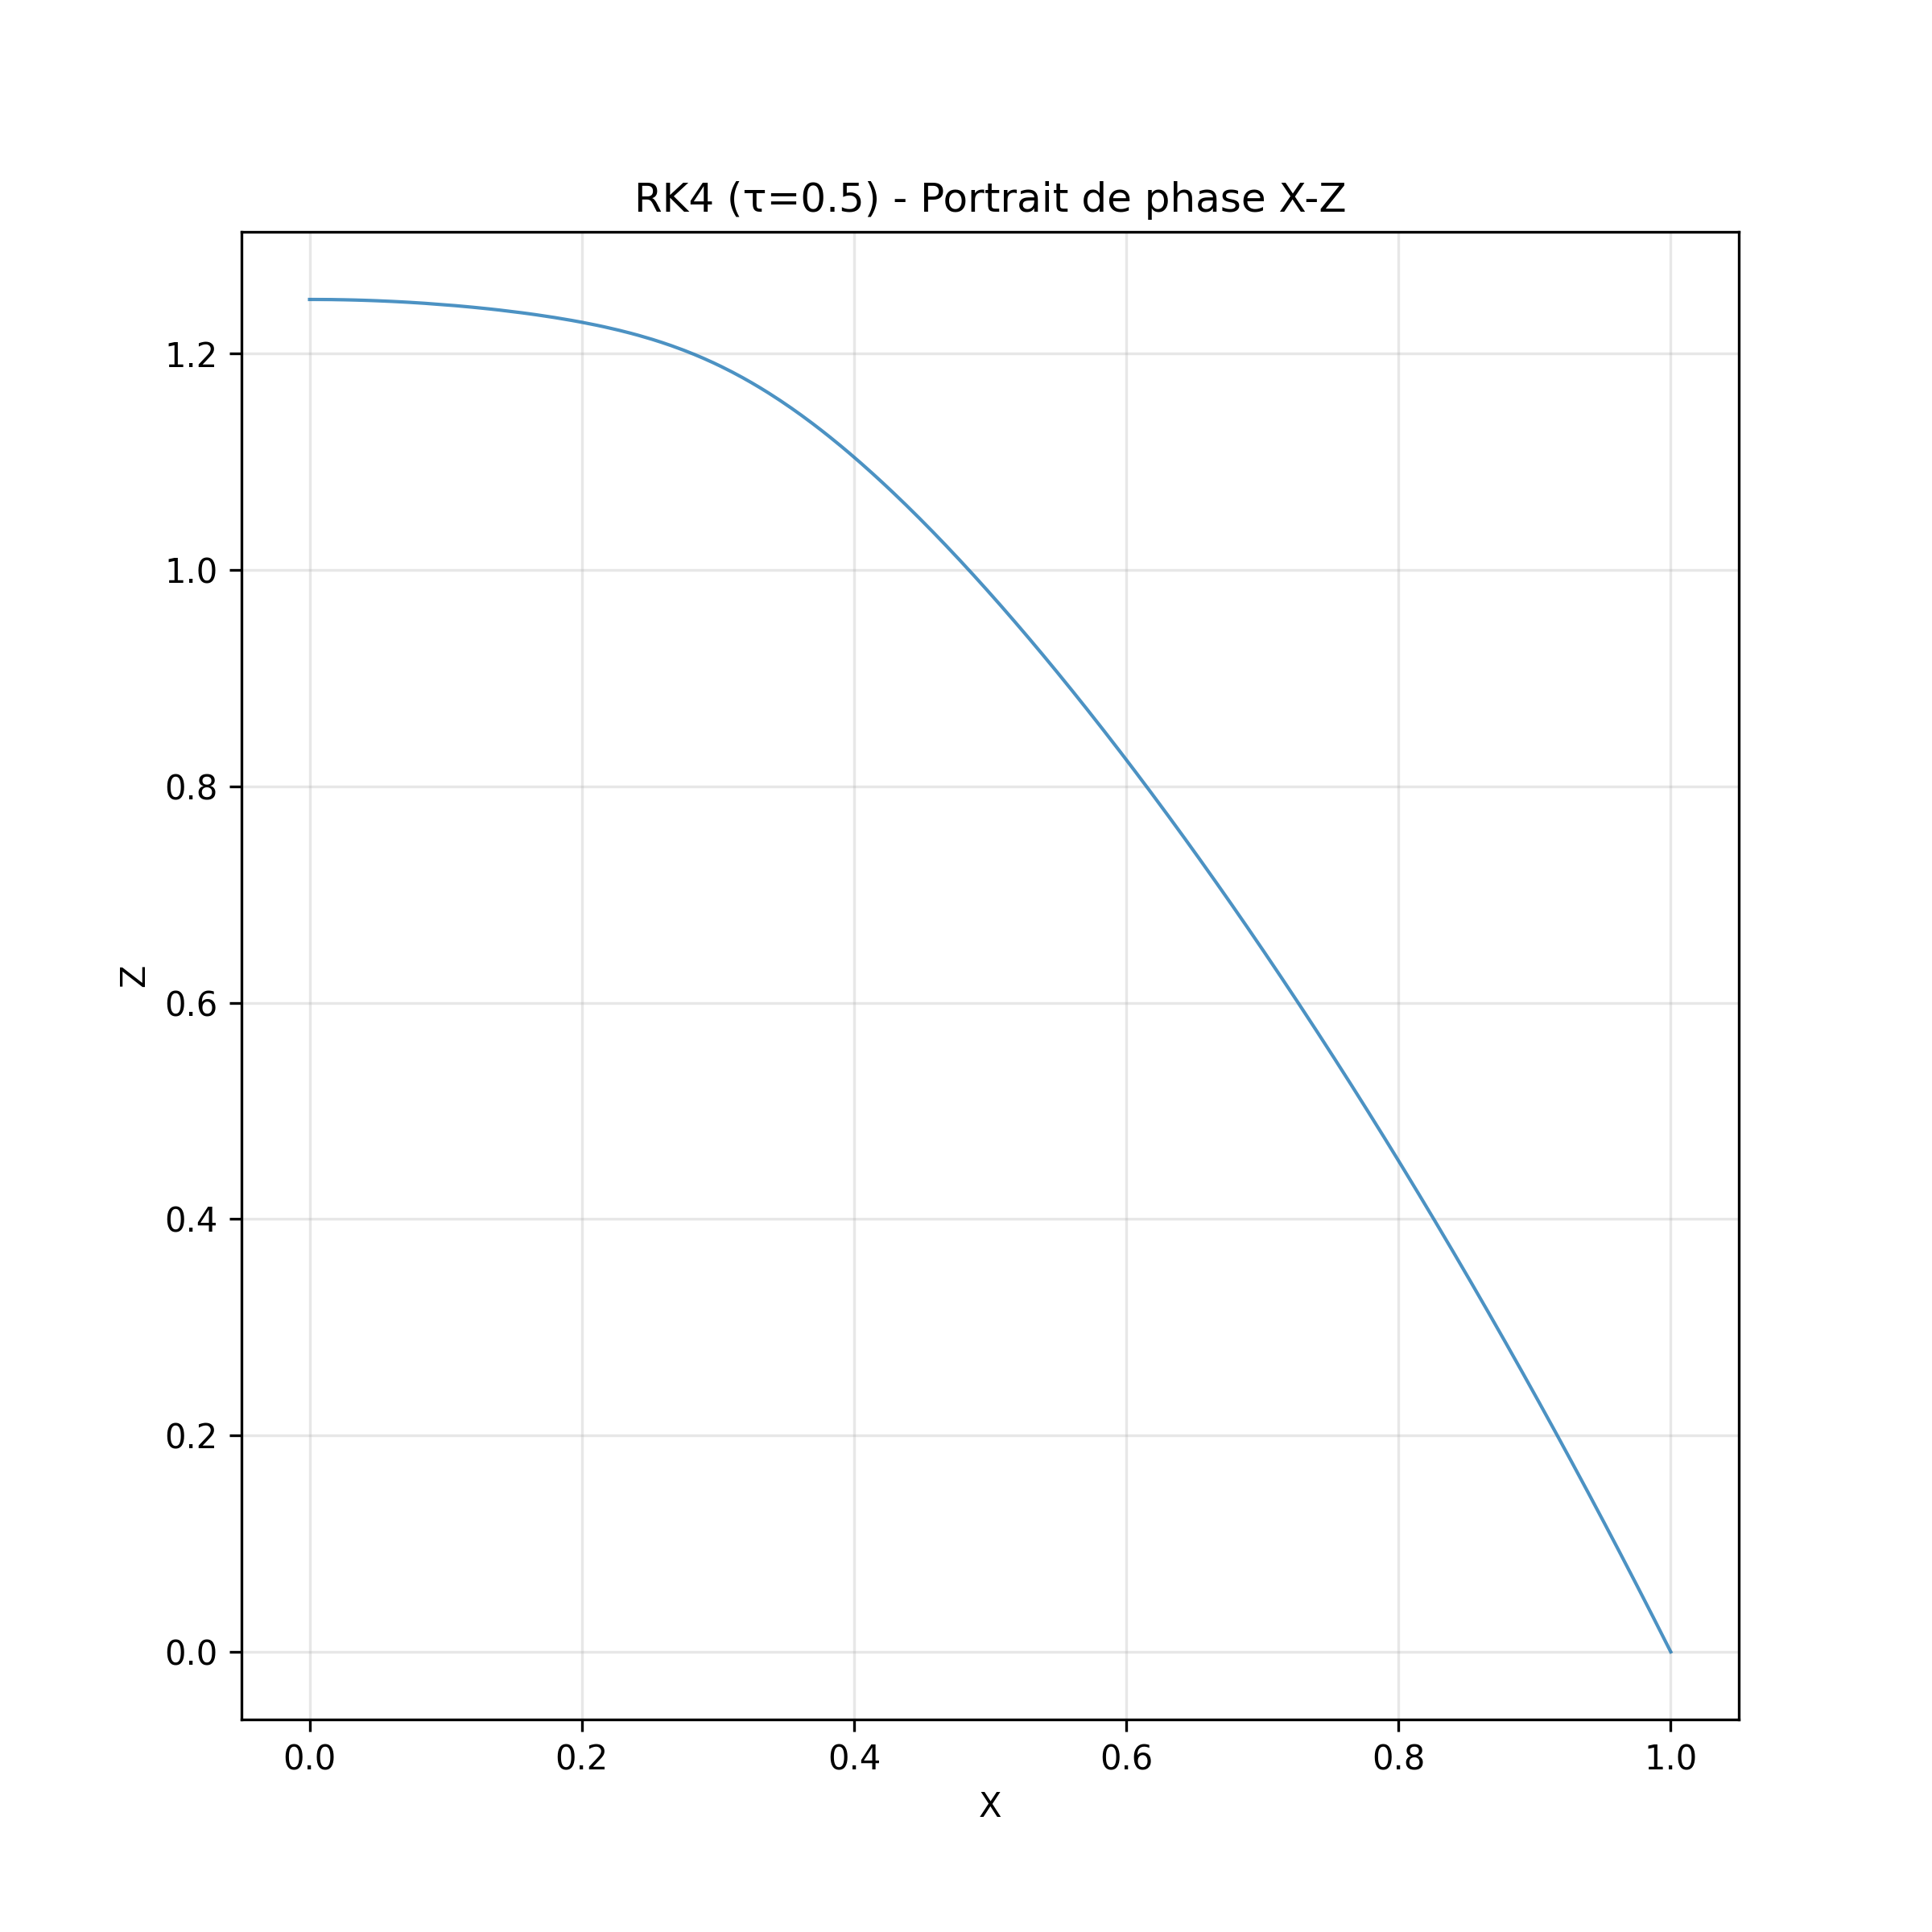
\includegraphics[width=\textwidth]{figures/rk4/rk4_tau0.5_phase}
        \caption{Portrait de phase}
    \end{subfigure}
    \caption{Dynamique pour $\tau$ = 0.5 : convergence vers un point fixe}
    \label{fig:rk4_tau0.5}
\end{figure}

\subsubsection{Marche Régulière ($\tau$ = 2.0)}
À $\tau$ = 2.0, le système présente des états stationnaires stables non triviaux.

En effet, on peut observer une stabilisation de la trajectoire autour de X non nulle et constante. 
\begin{figure}[H]
    \centering
    \begin{subfigure}[b]{0.5\textwidth}
        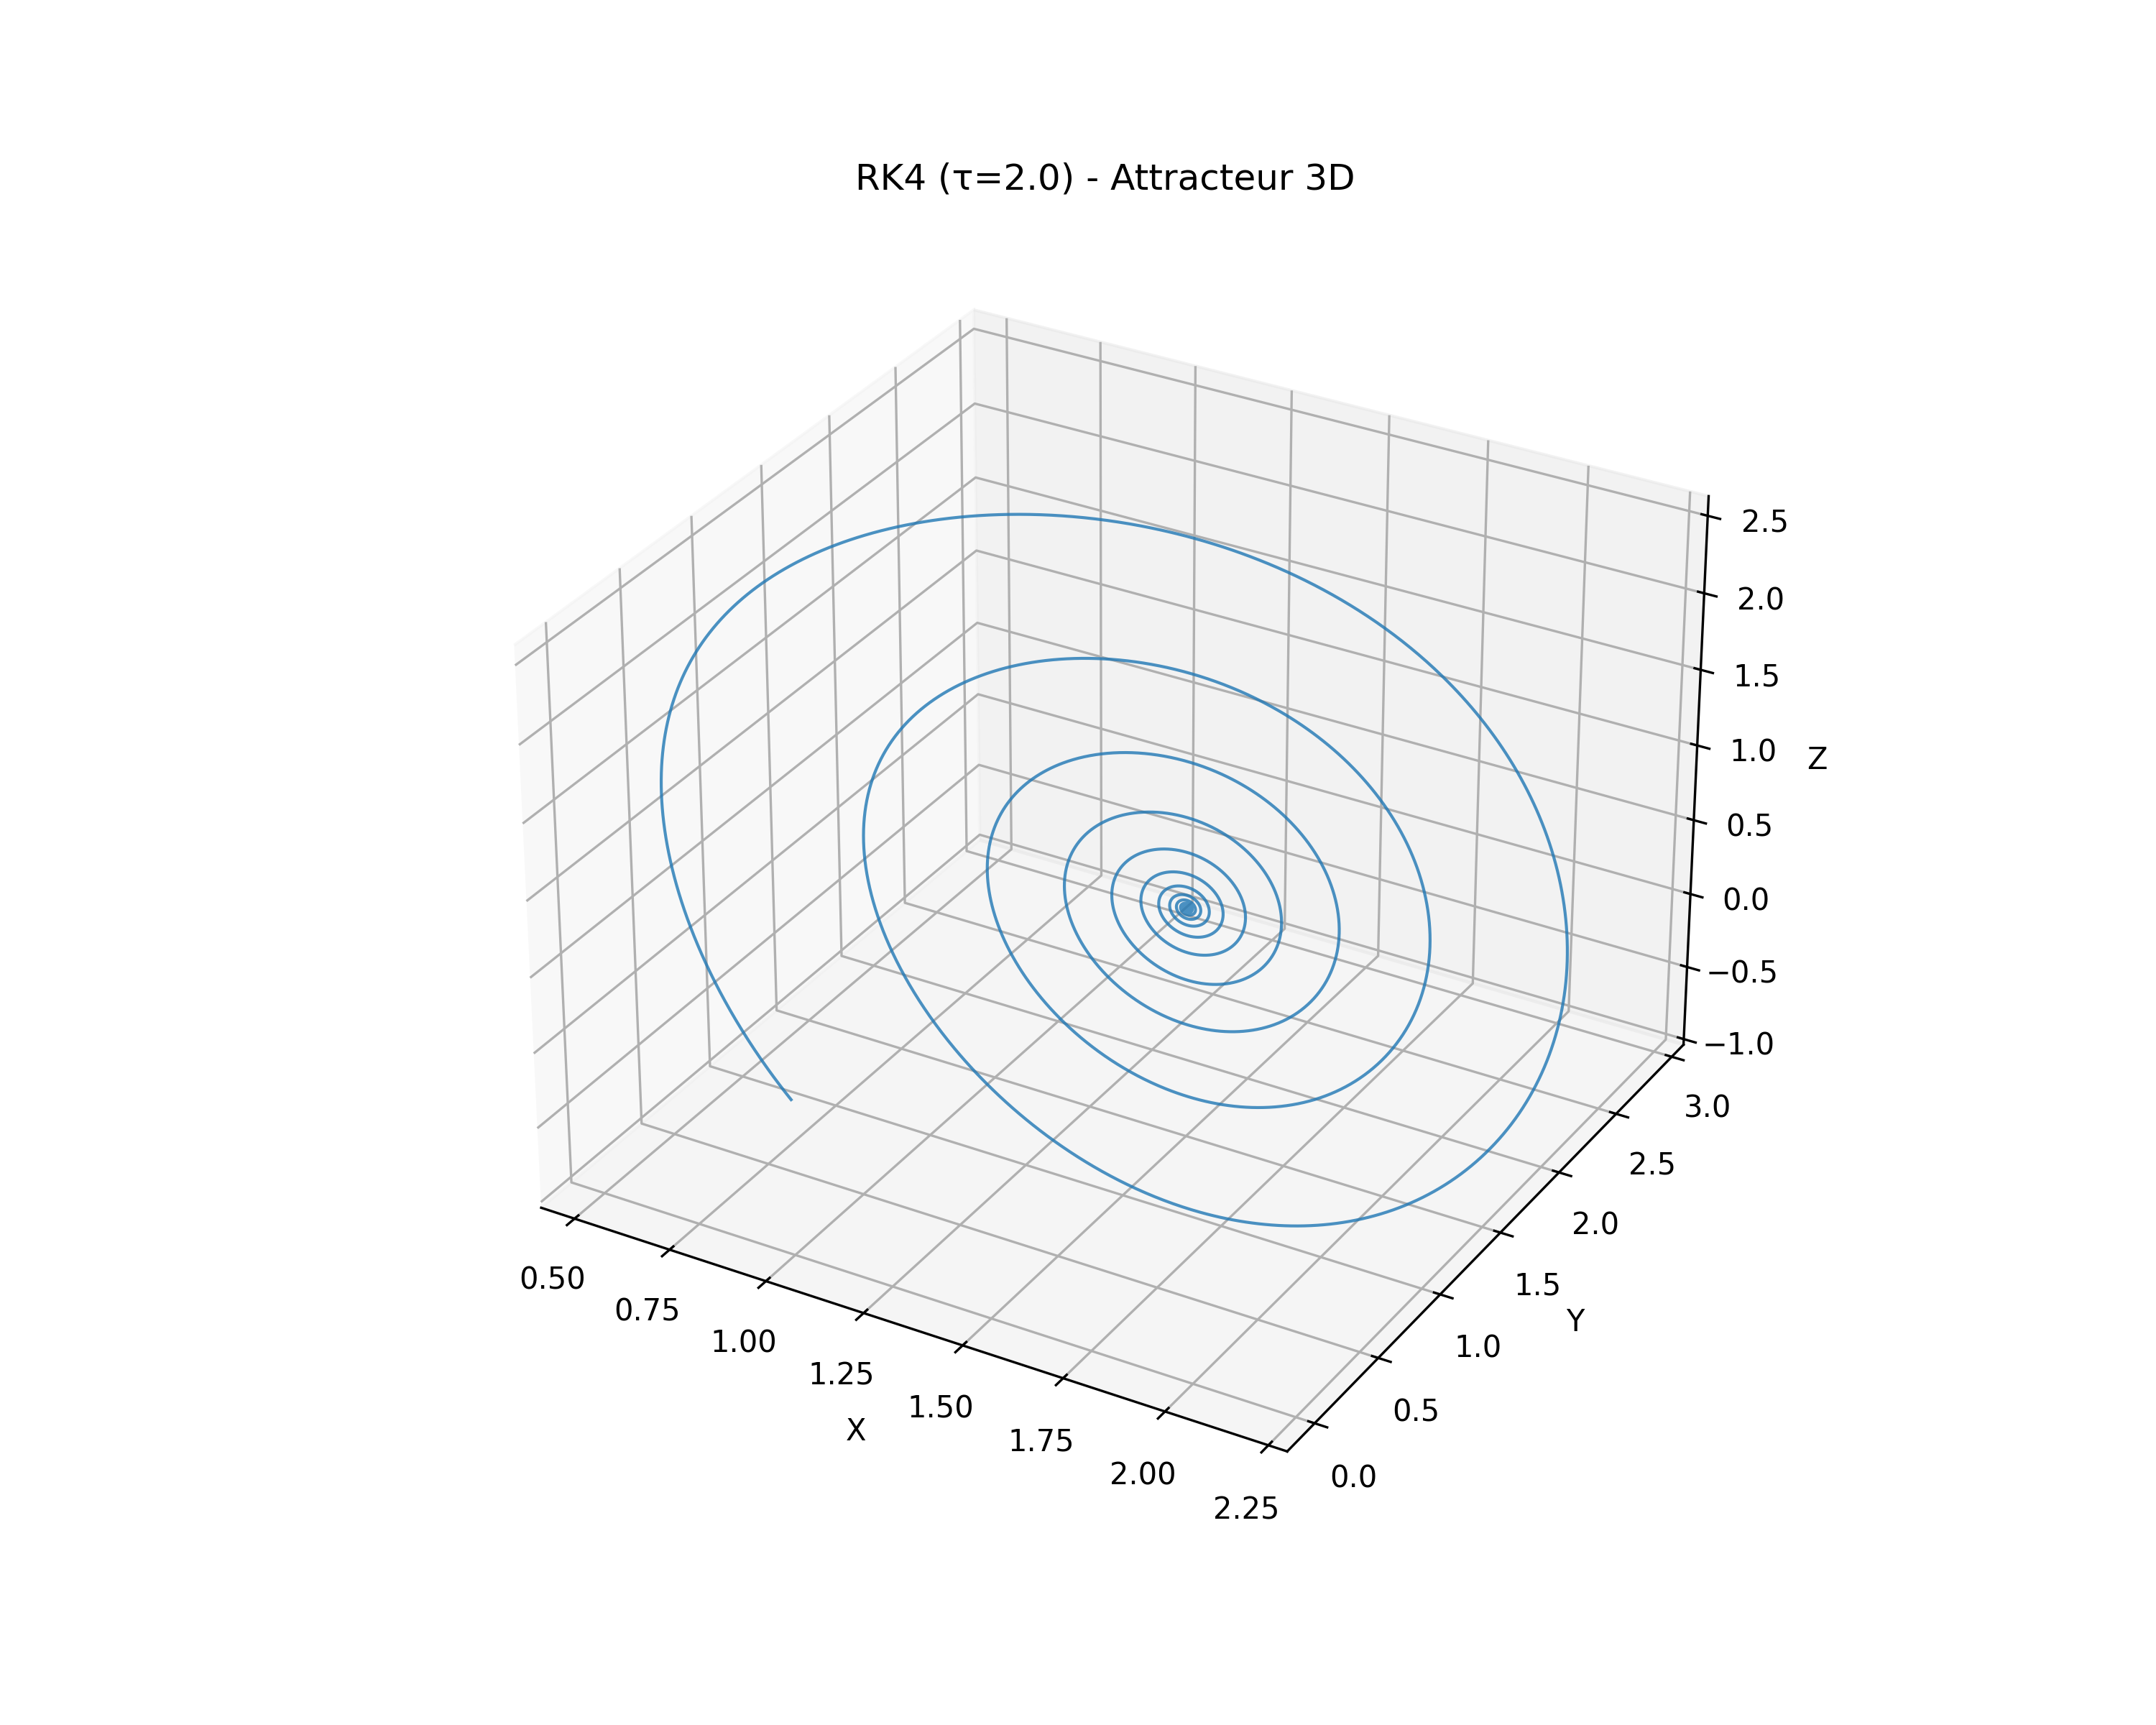
\includegraphics[width=\textwidth]{figures/rk4/rk4_tau2.0_3d}
        \caption{Trajectoire 3D : Trajectoire convergeant vers un point fixe non trivial}
    \end{subfigure}
    \begin{subfigure}[b]{0.4\textwidth}
        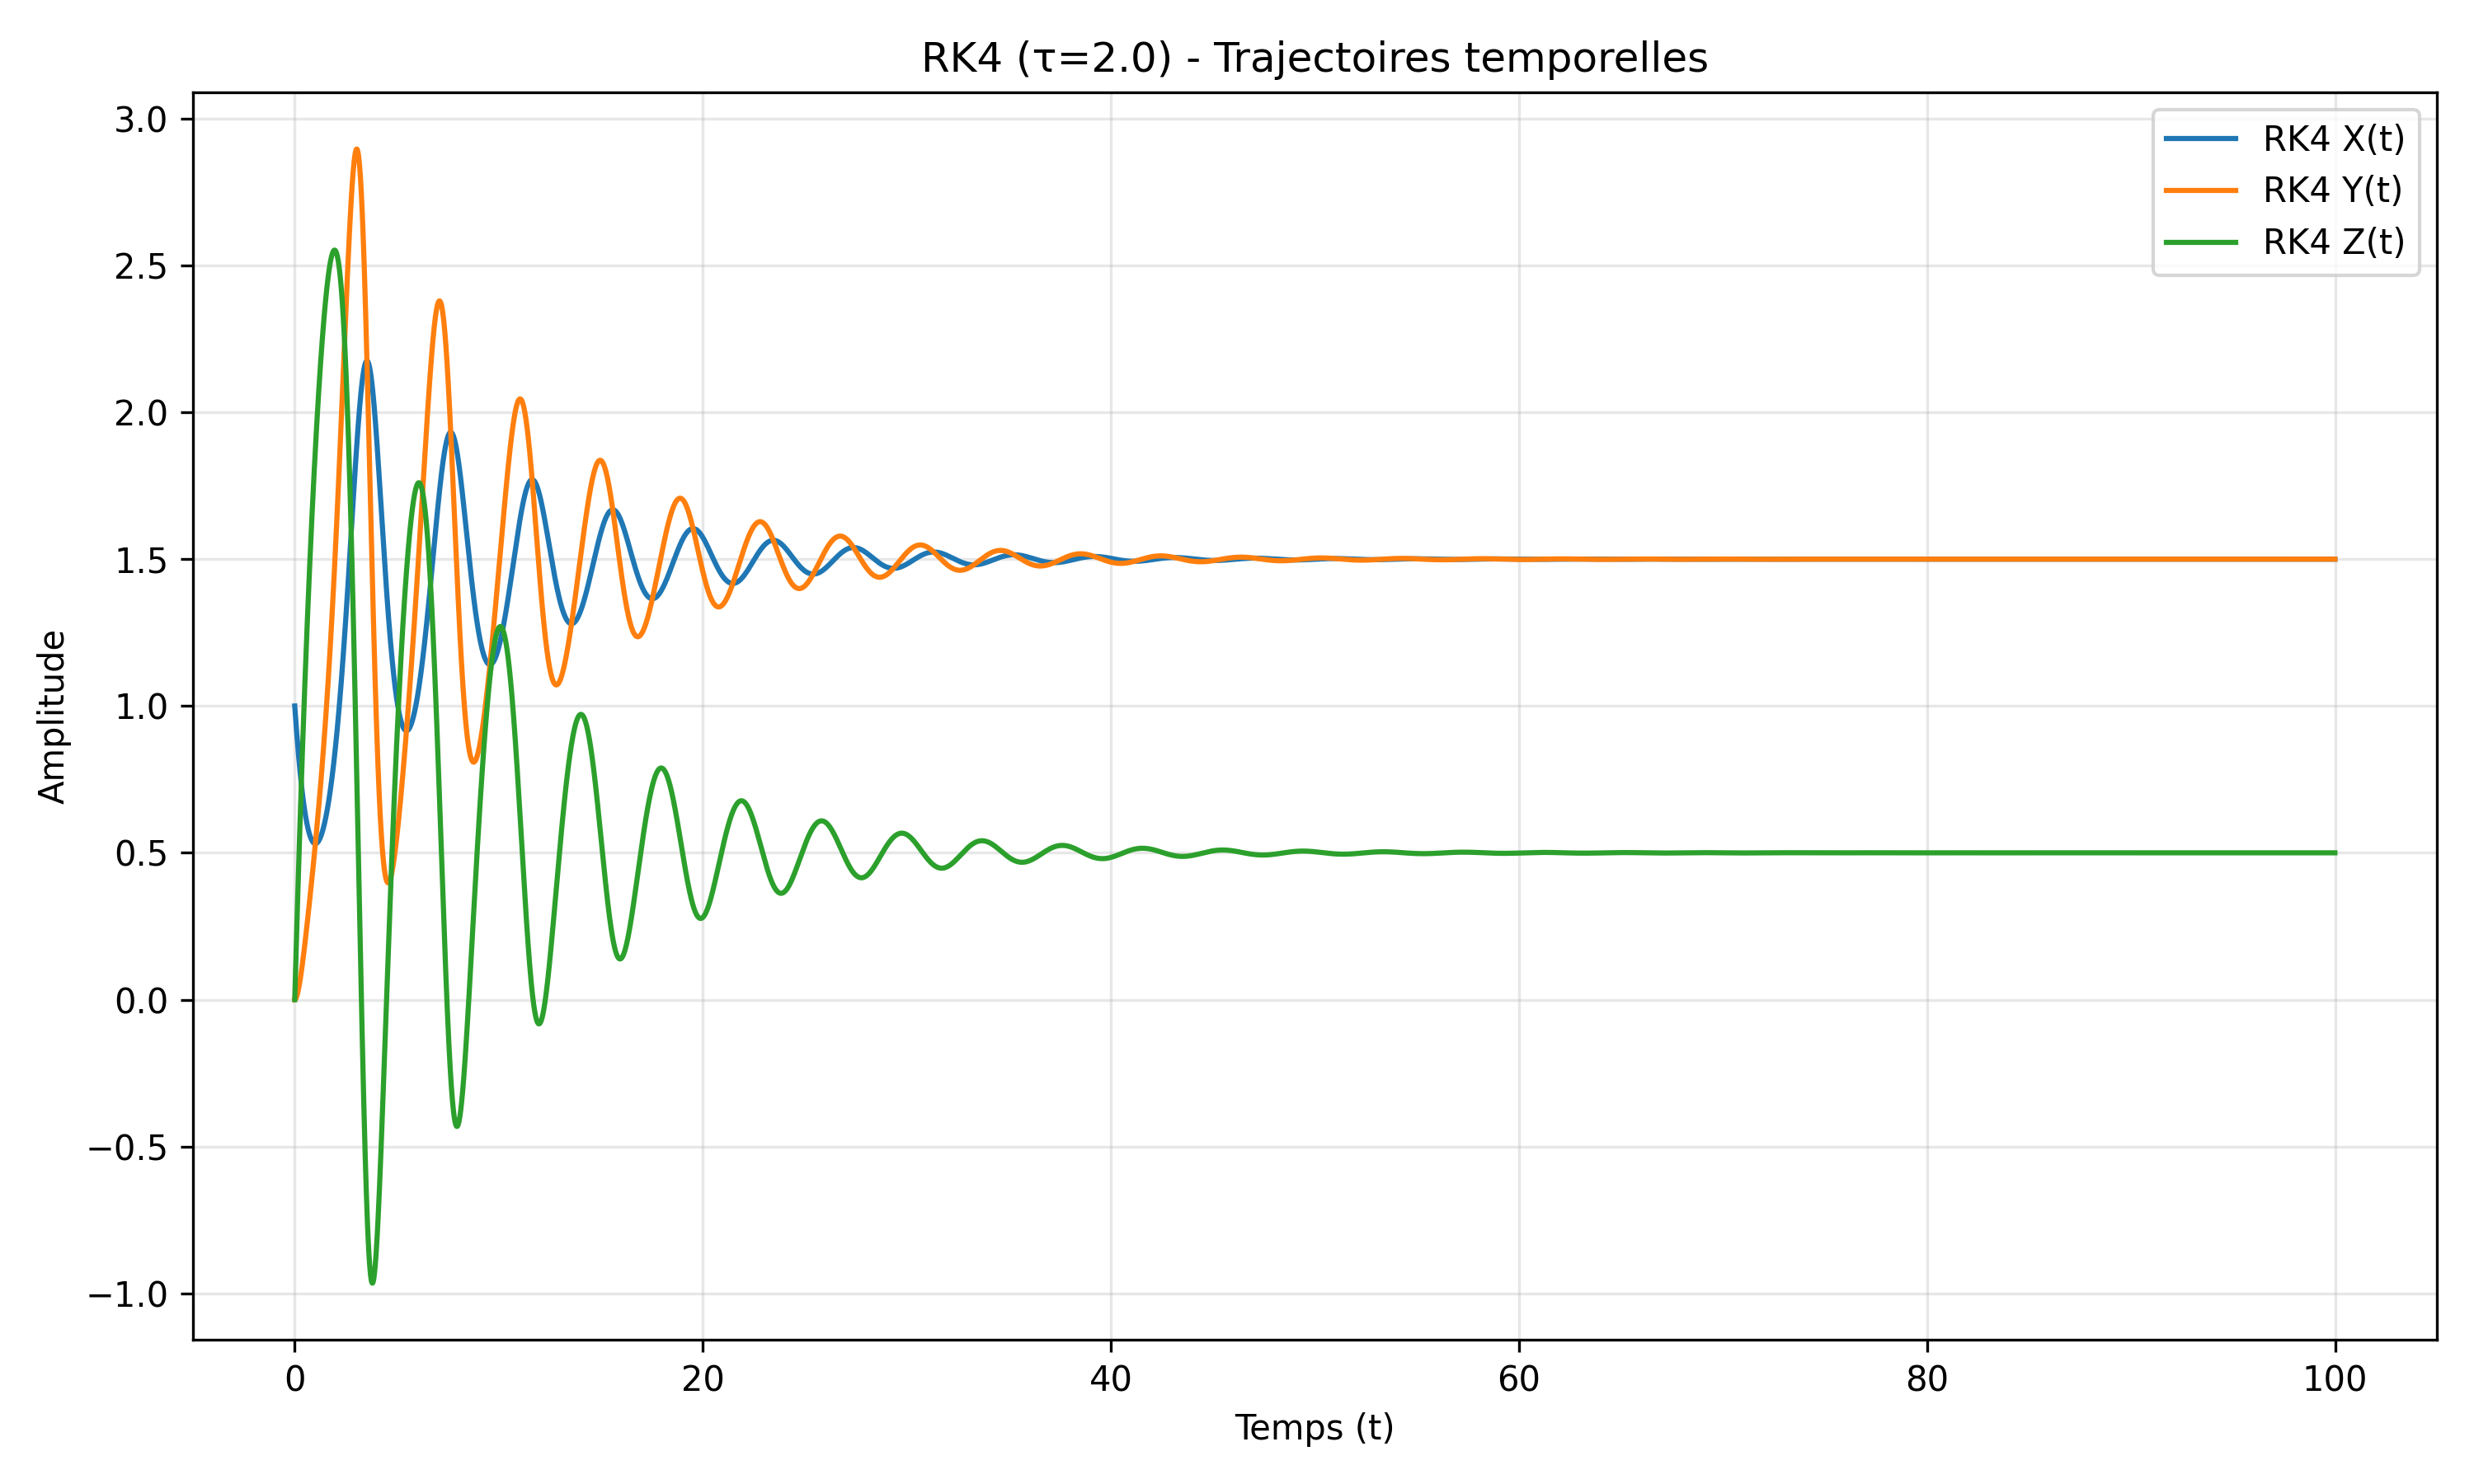
\includegraphics[width=\textwidth]{figures/rk4/rk4_tau2.0_time}
        \caption{Évolution temporelle : X et Y se stabilisent à des valeurs non-nulles constantes, Z reste stable}
    \end{subfigure}
    \begin{subfigure}[b]{0.3\textwidth}
        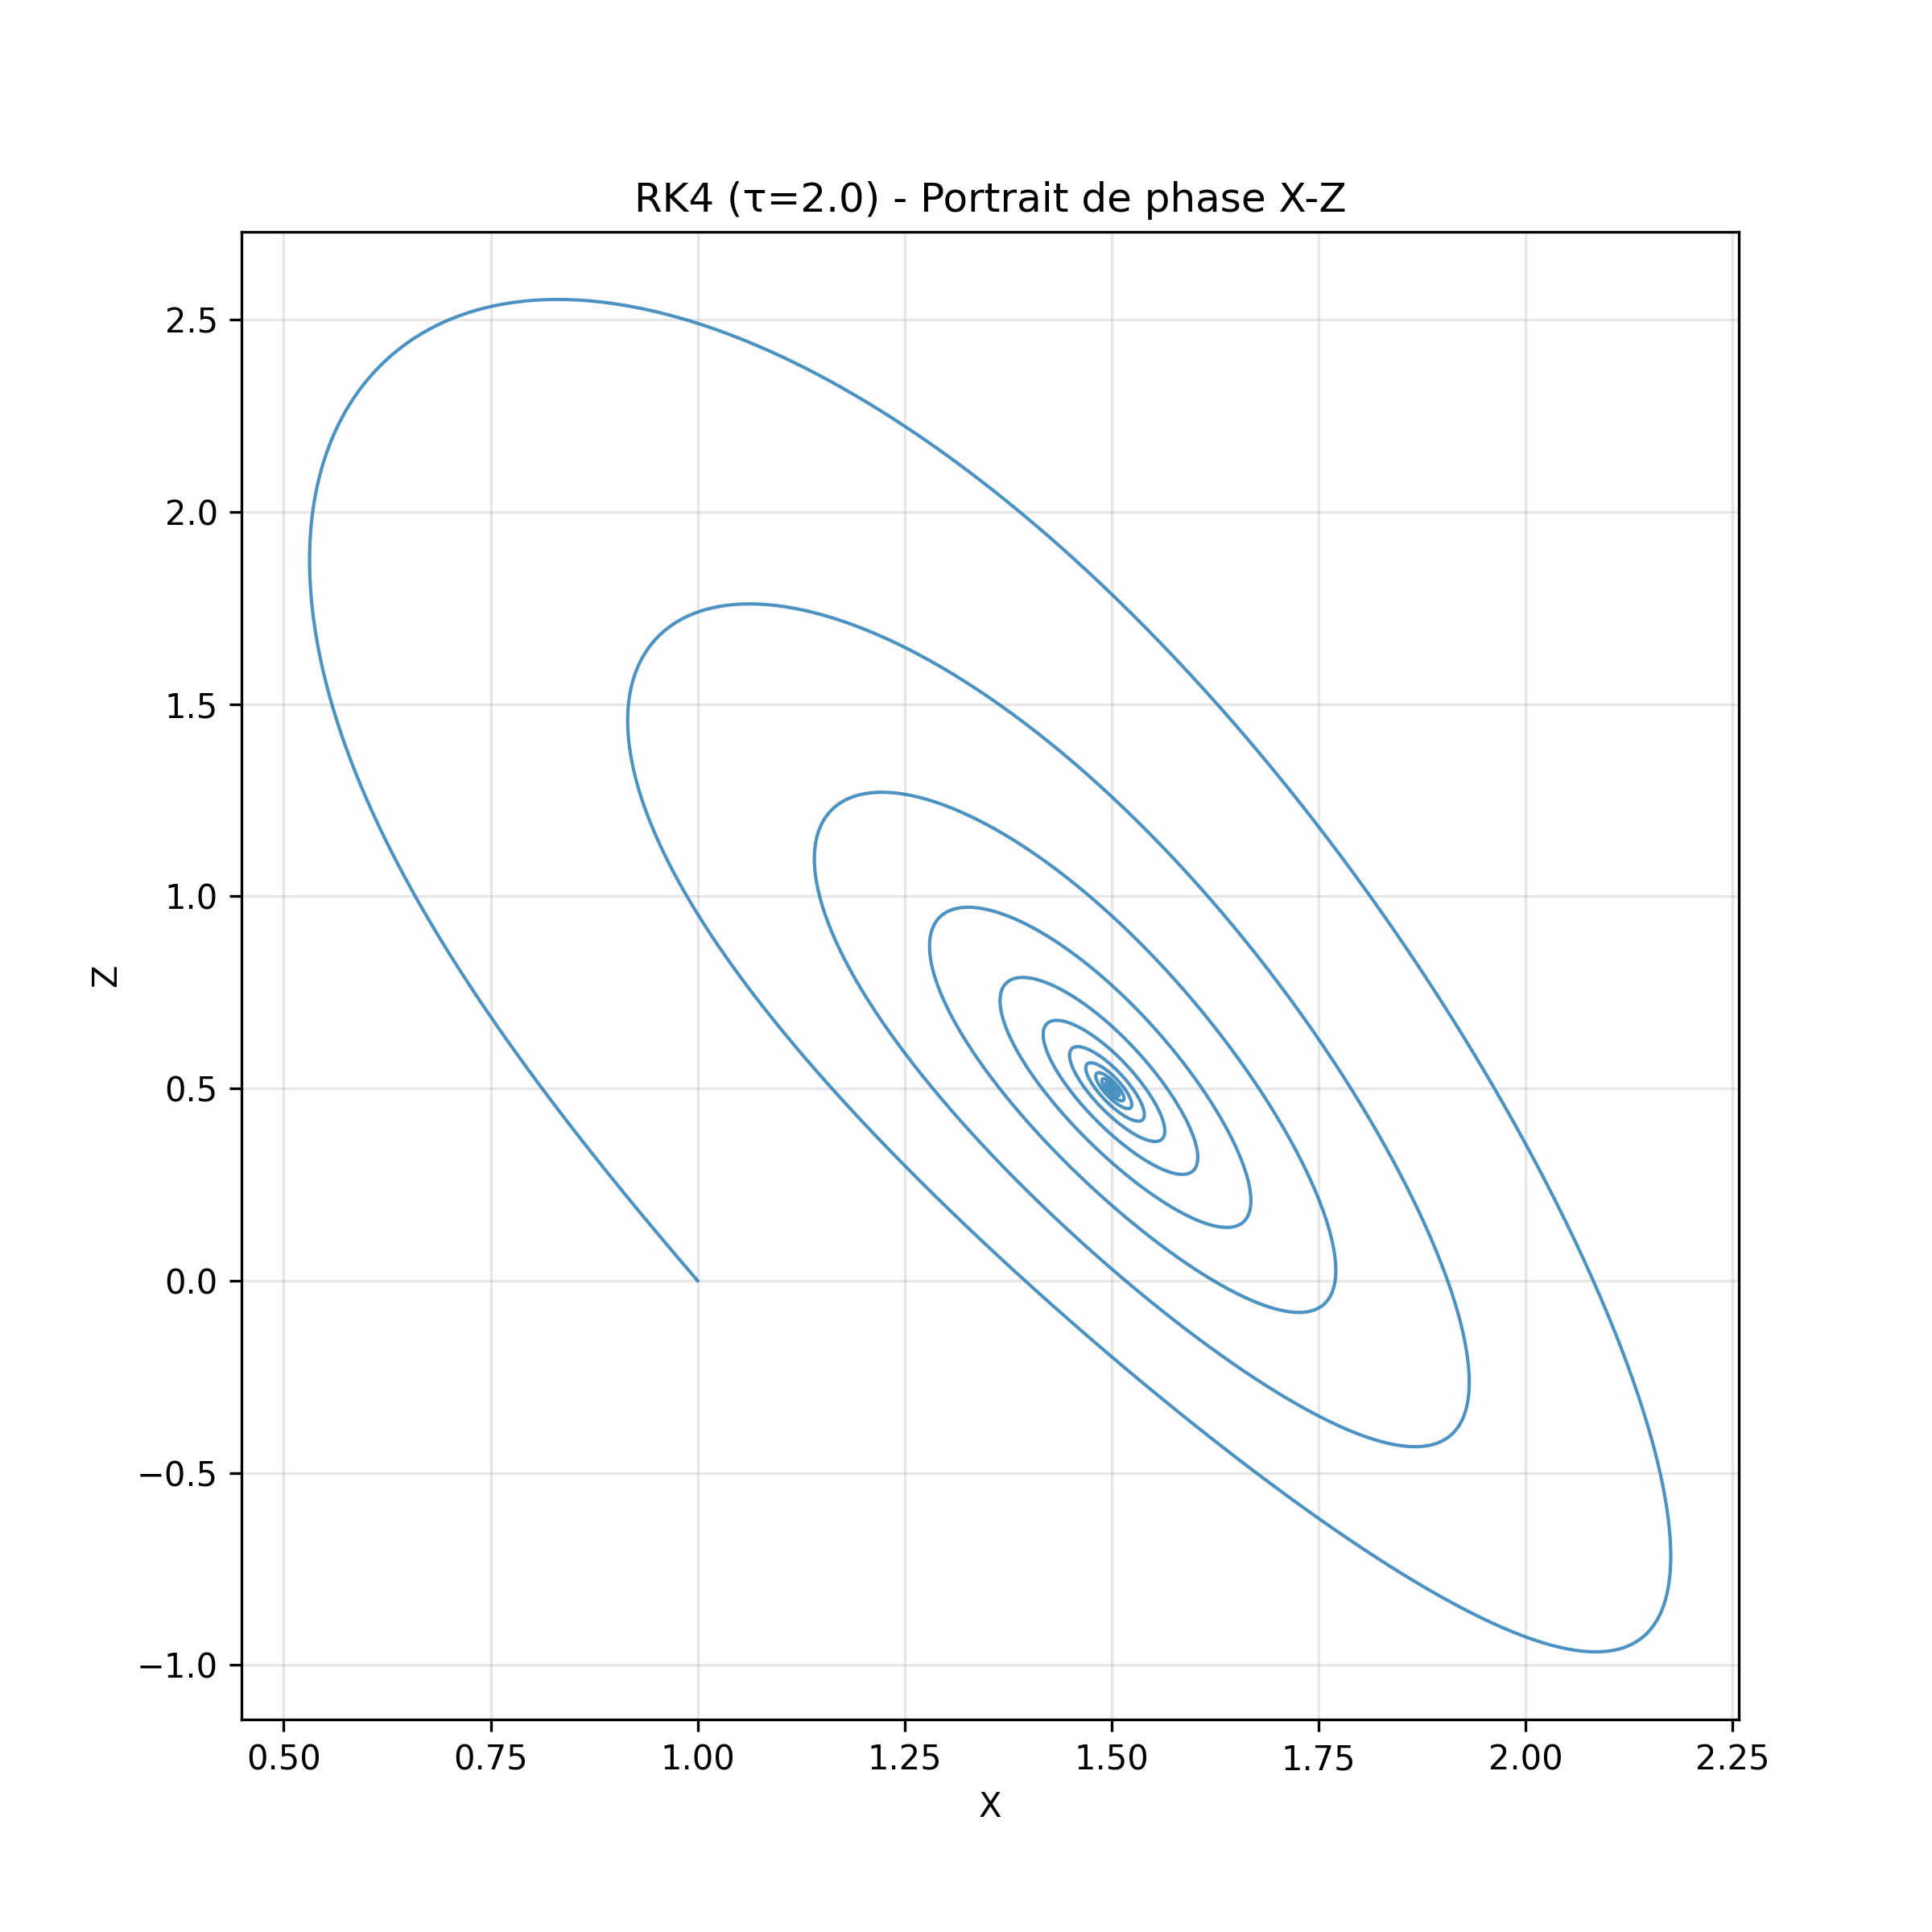
\includegraphics[width=\textwidth]{figures/rk4/rk4_tau2.0_phase}
        \caption{Portrait de phase}
    \end{subfigure}
    \caption{Dynamique pour $\tau$ = 2.0 : états stationnaires stables}
    \label{fig:rk4_tau2.0}
\end{figure}

\subsubsection{Marche Chaotique ($\tau$ = 5.0)}
À $\tau$ = 5.0, on observe l'apparition d'oscillations complexes.

Aucun motif régulier ou périodique n'est observable clairement dans la dynamique du système.
\begin{figure}[H]
    \centering
    \begin{subfigure}[b]{0.5\textwidth}
        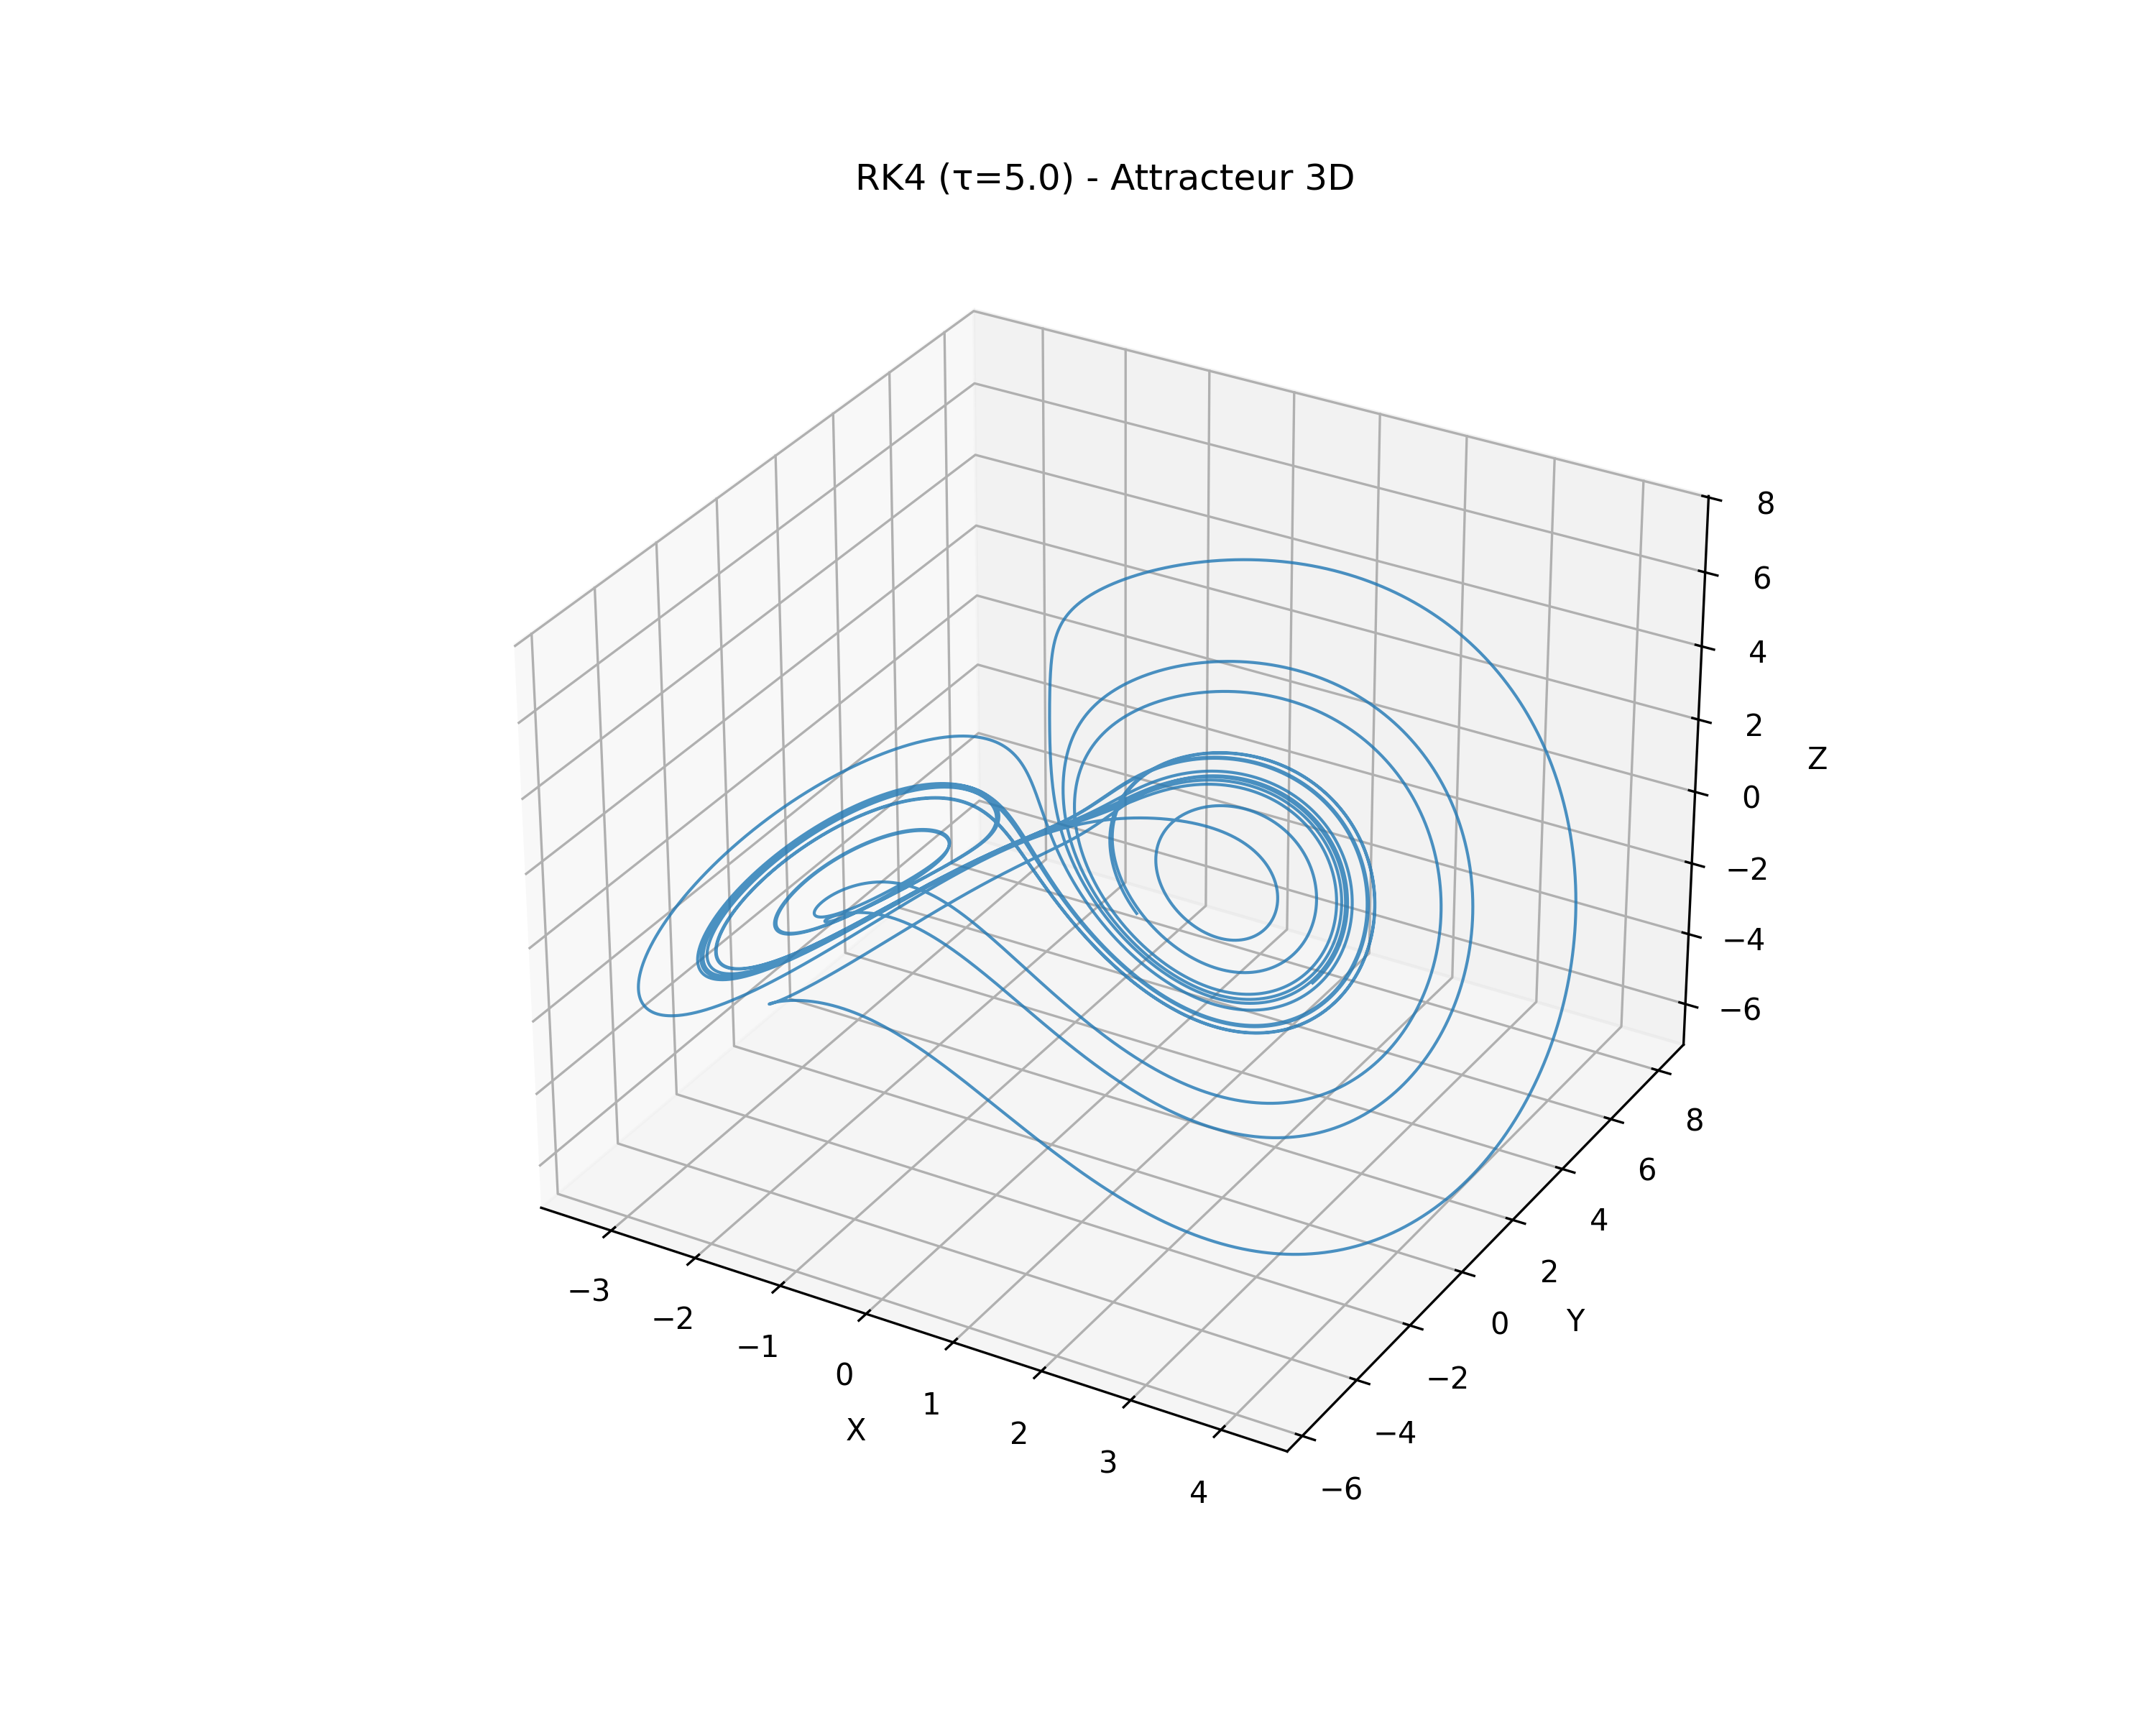
\includegraphics[width=\textwidth]{figures/rk4/rk4_tau5.0_3d}
        \caption{Trajectoire 3D : Attracteur étrange tridimensionnel avec structure complexe}
    \end{subfigure}
    \begin{subfigure}[b]{0.4\textwidth}
        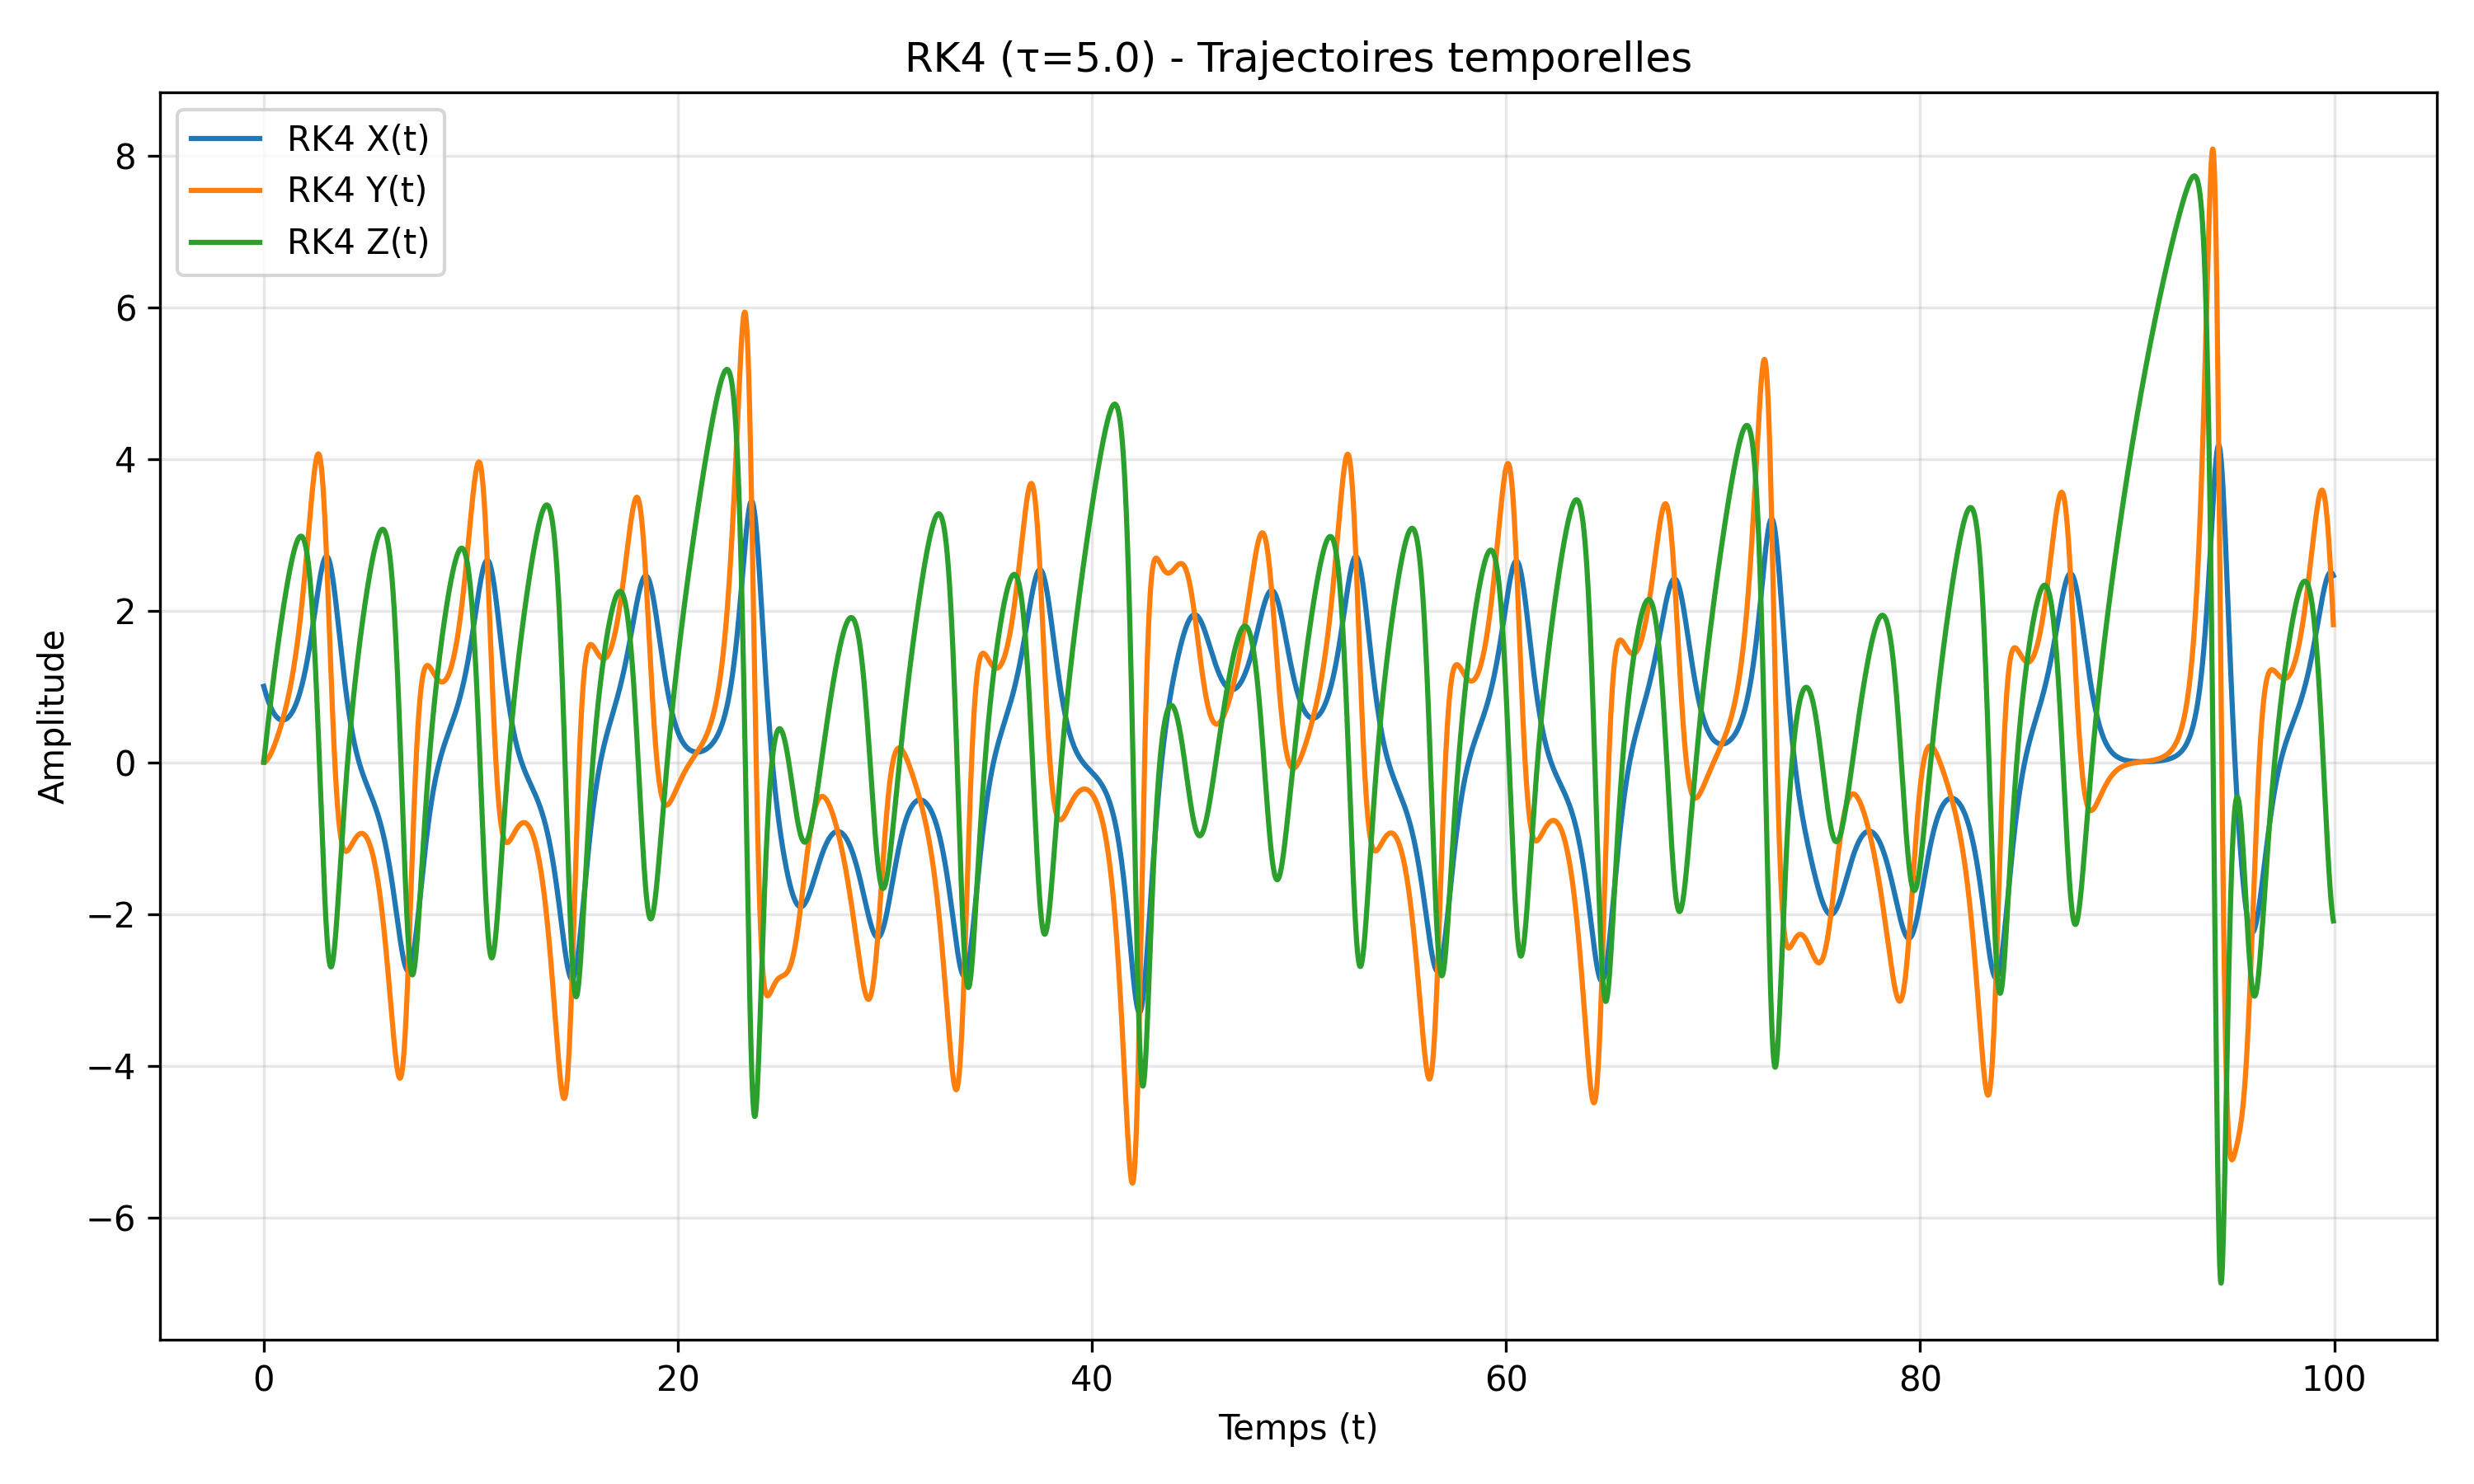
\includegraphics[width=\textwidth]{figures/rk4/rk4_tau5.0_time}
        \caption{Évolution temporelle : Fortes oscillations irrégulières de toutes les variables }
    \end{subfigure}
    \begin{subfigure}[b]{0.3\textwidth}
        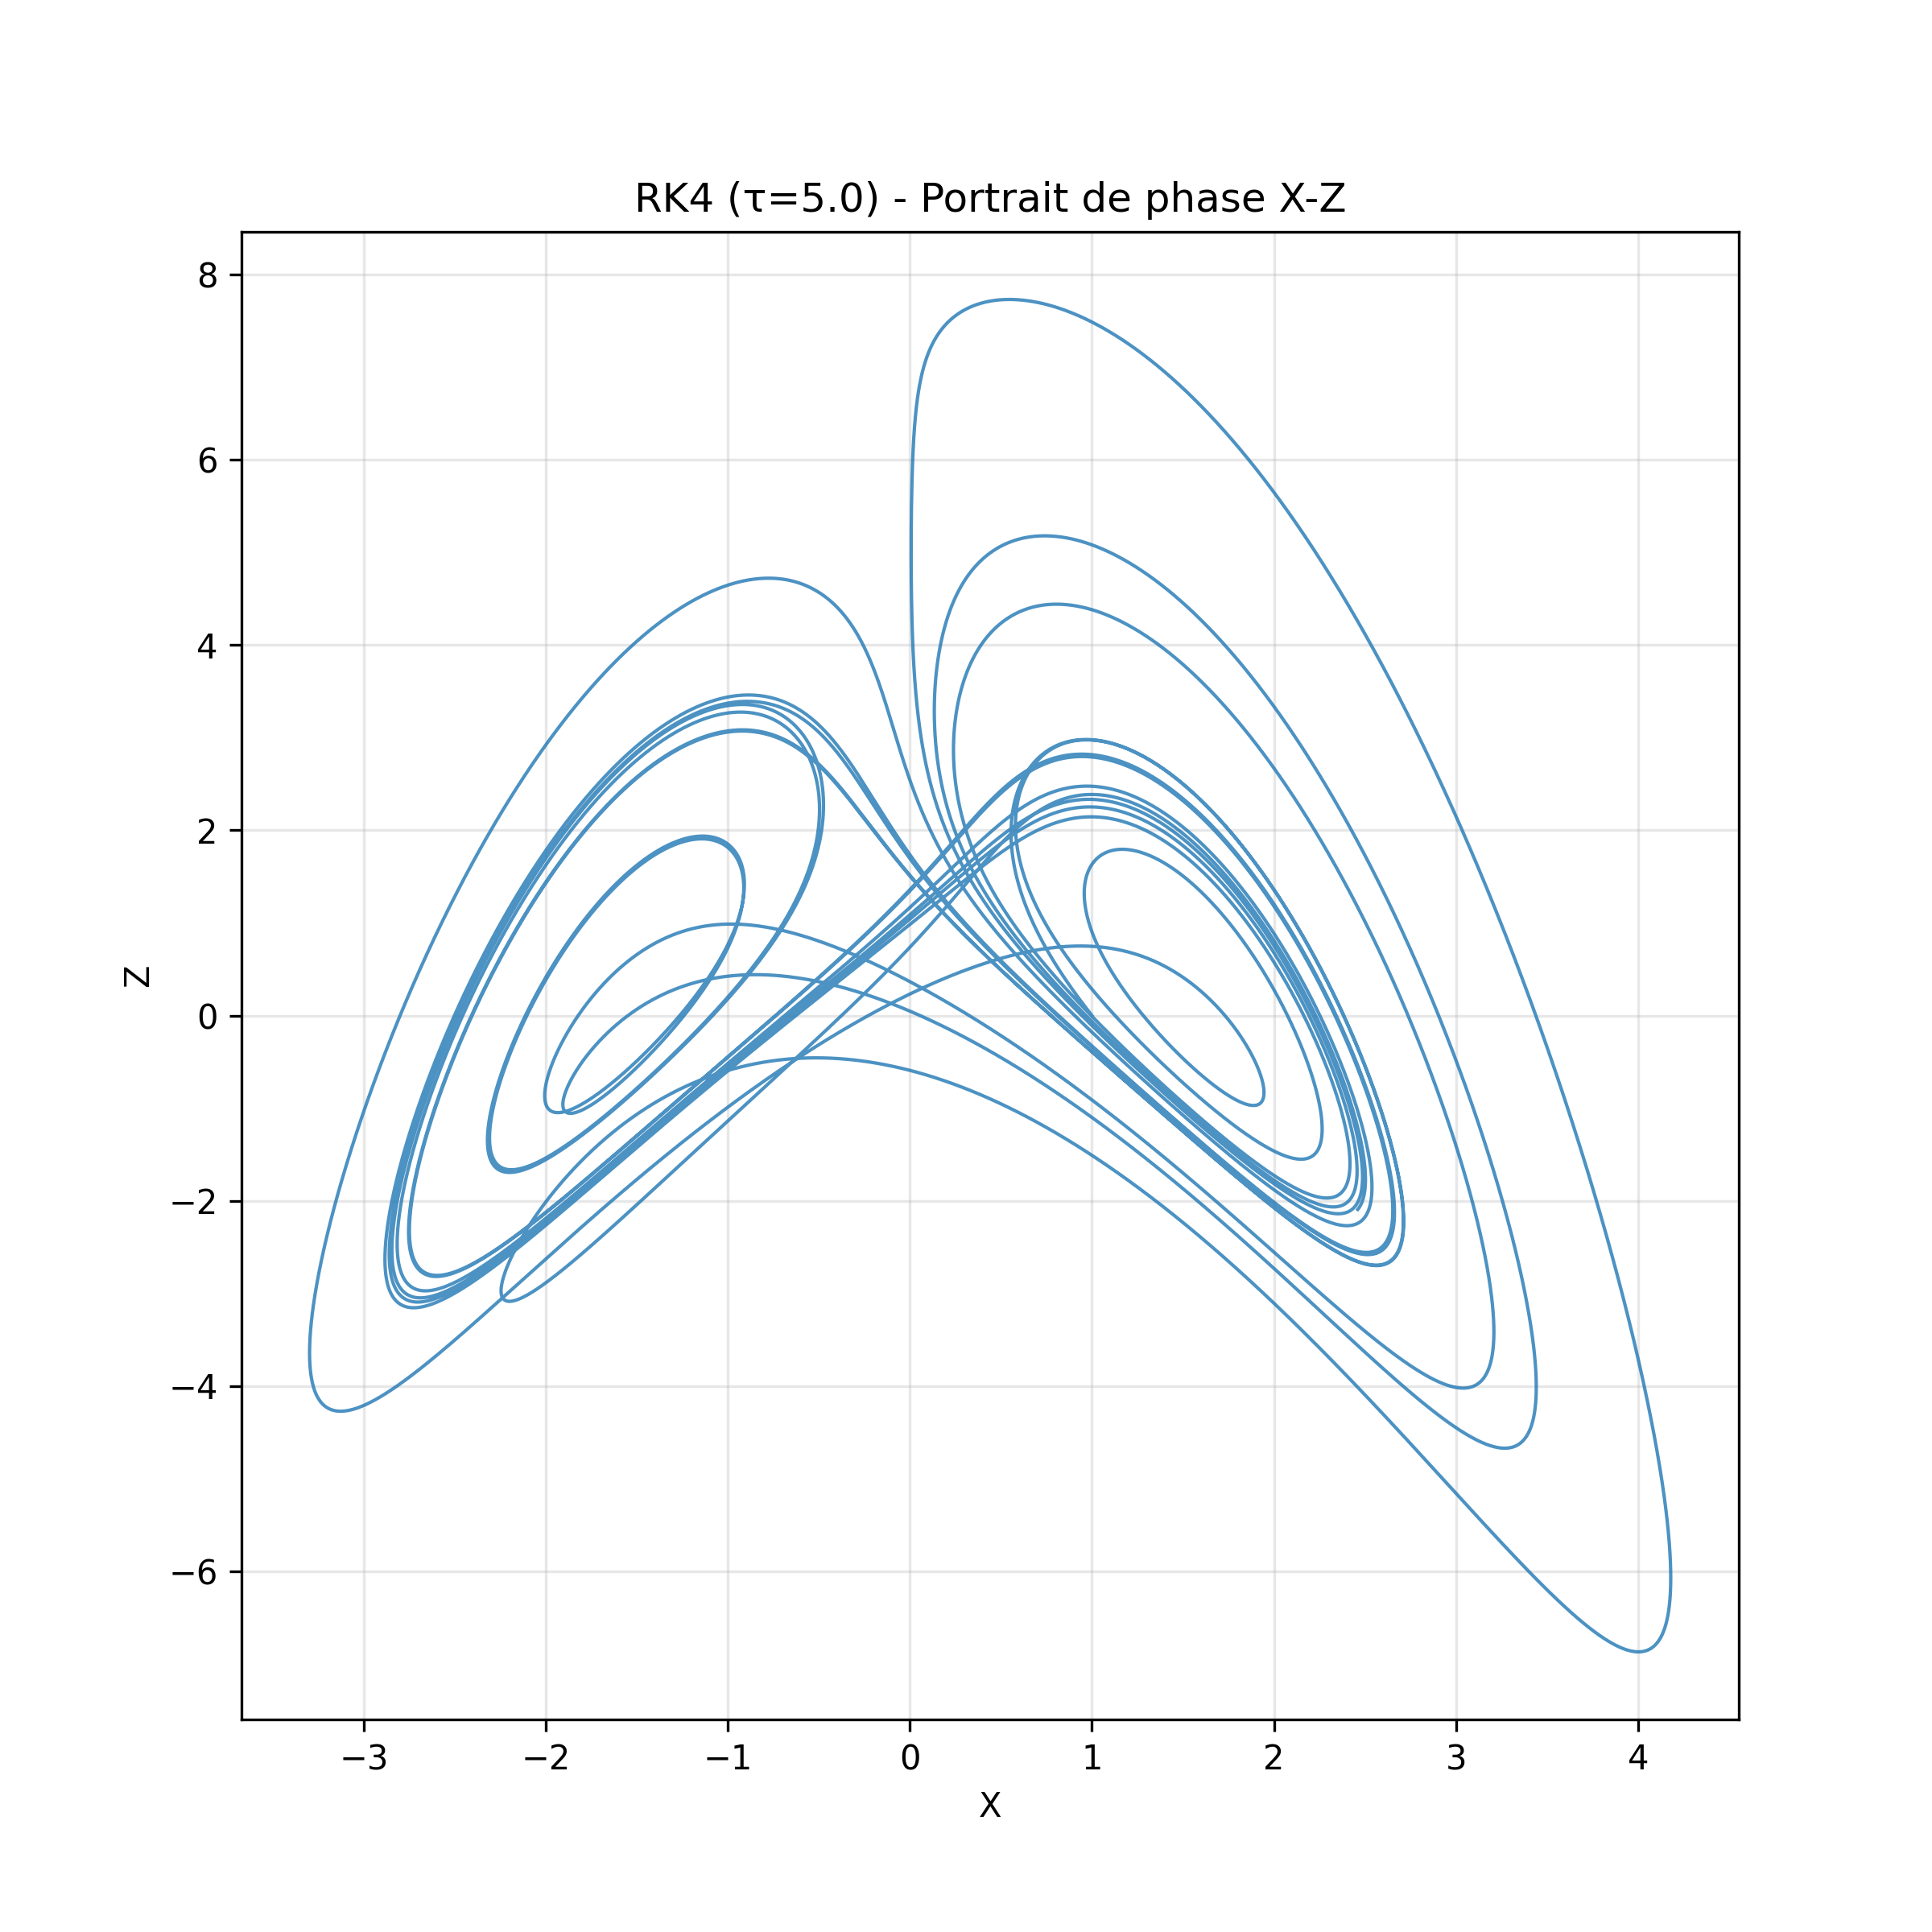
\includegraphics[width=\textwidth]{figures/rk4/rk4_tau5.0_phase}
        \caption{Portrait de phase : Attracteur étrange avec structure fractale complexe.}
    \end{subfigure}
    \caption{Dynamique pour $\tau$ = 5.0 : oscillations complexes}
    \label{fig:rk4_tau5.0}
\end{figure}

\subsubsection{Oscillations avec Dérive ($\tau$ = 8.9)}
Pour $\tau$ = 8.9, le système entre dans un régime pleinement chaotique.

Les oscillations sont quasi-périodiques avec une dérive progressive, et les motifs sont de plus en plus complexes. La structure est plus organisé que le scénario chaotique précédent, mais moins stable que le scénario de 
\begin{figure}[H]
    \centering
    \begin{subfigure}[b]{0.5\textwidth}
        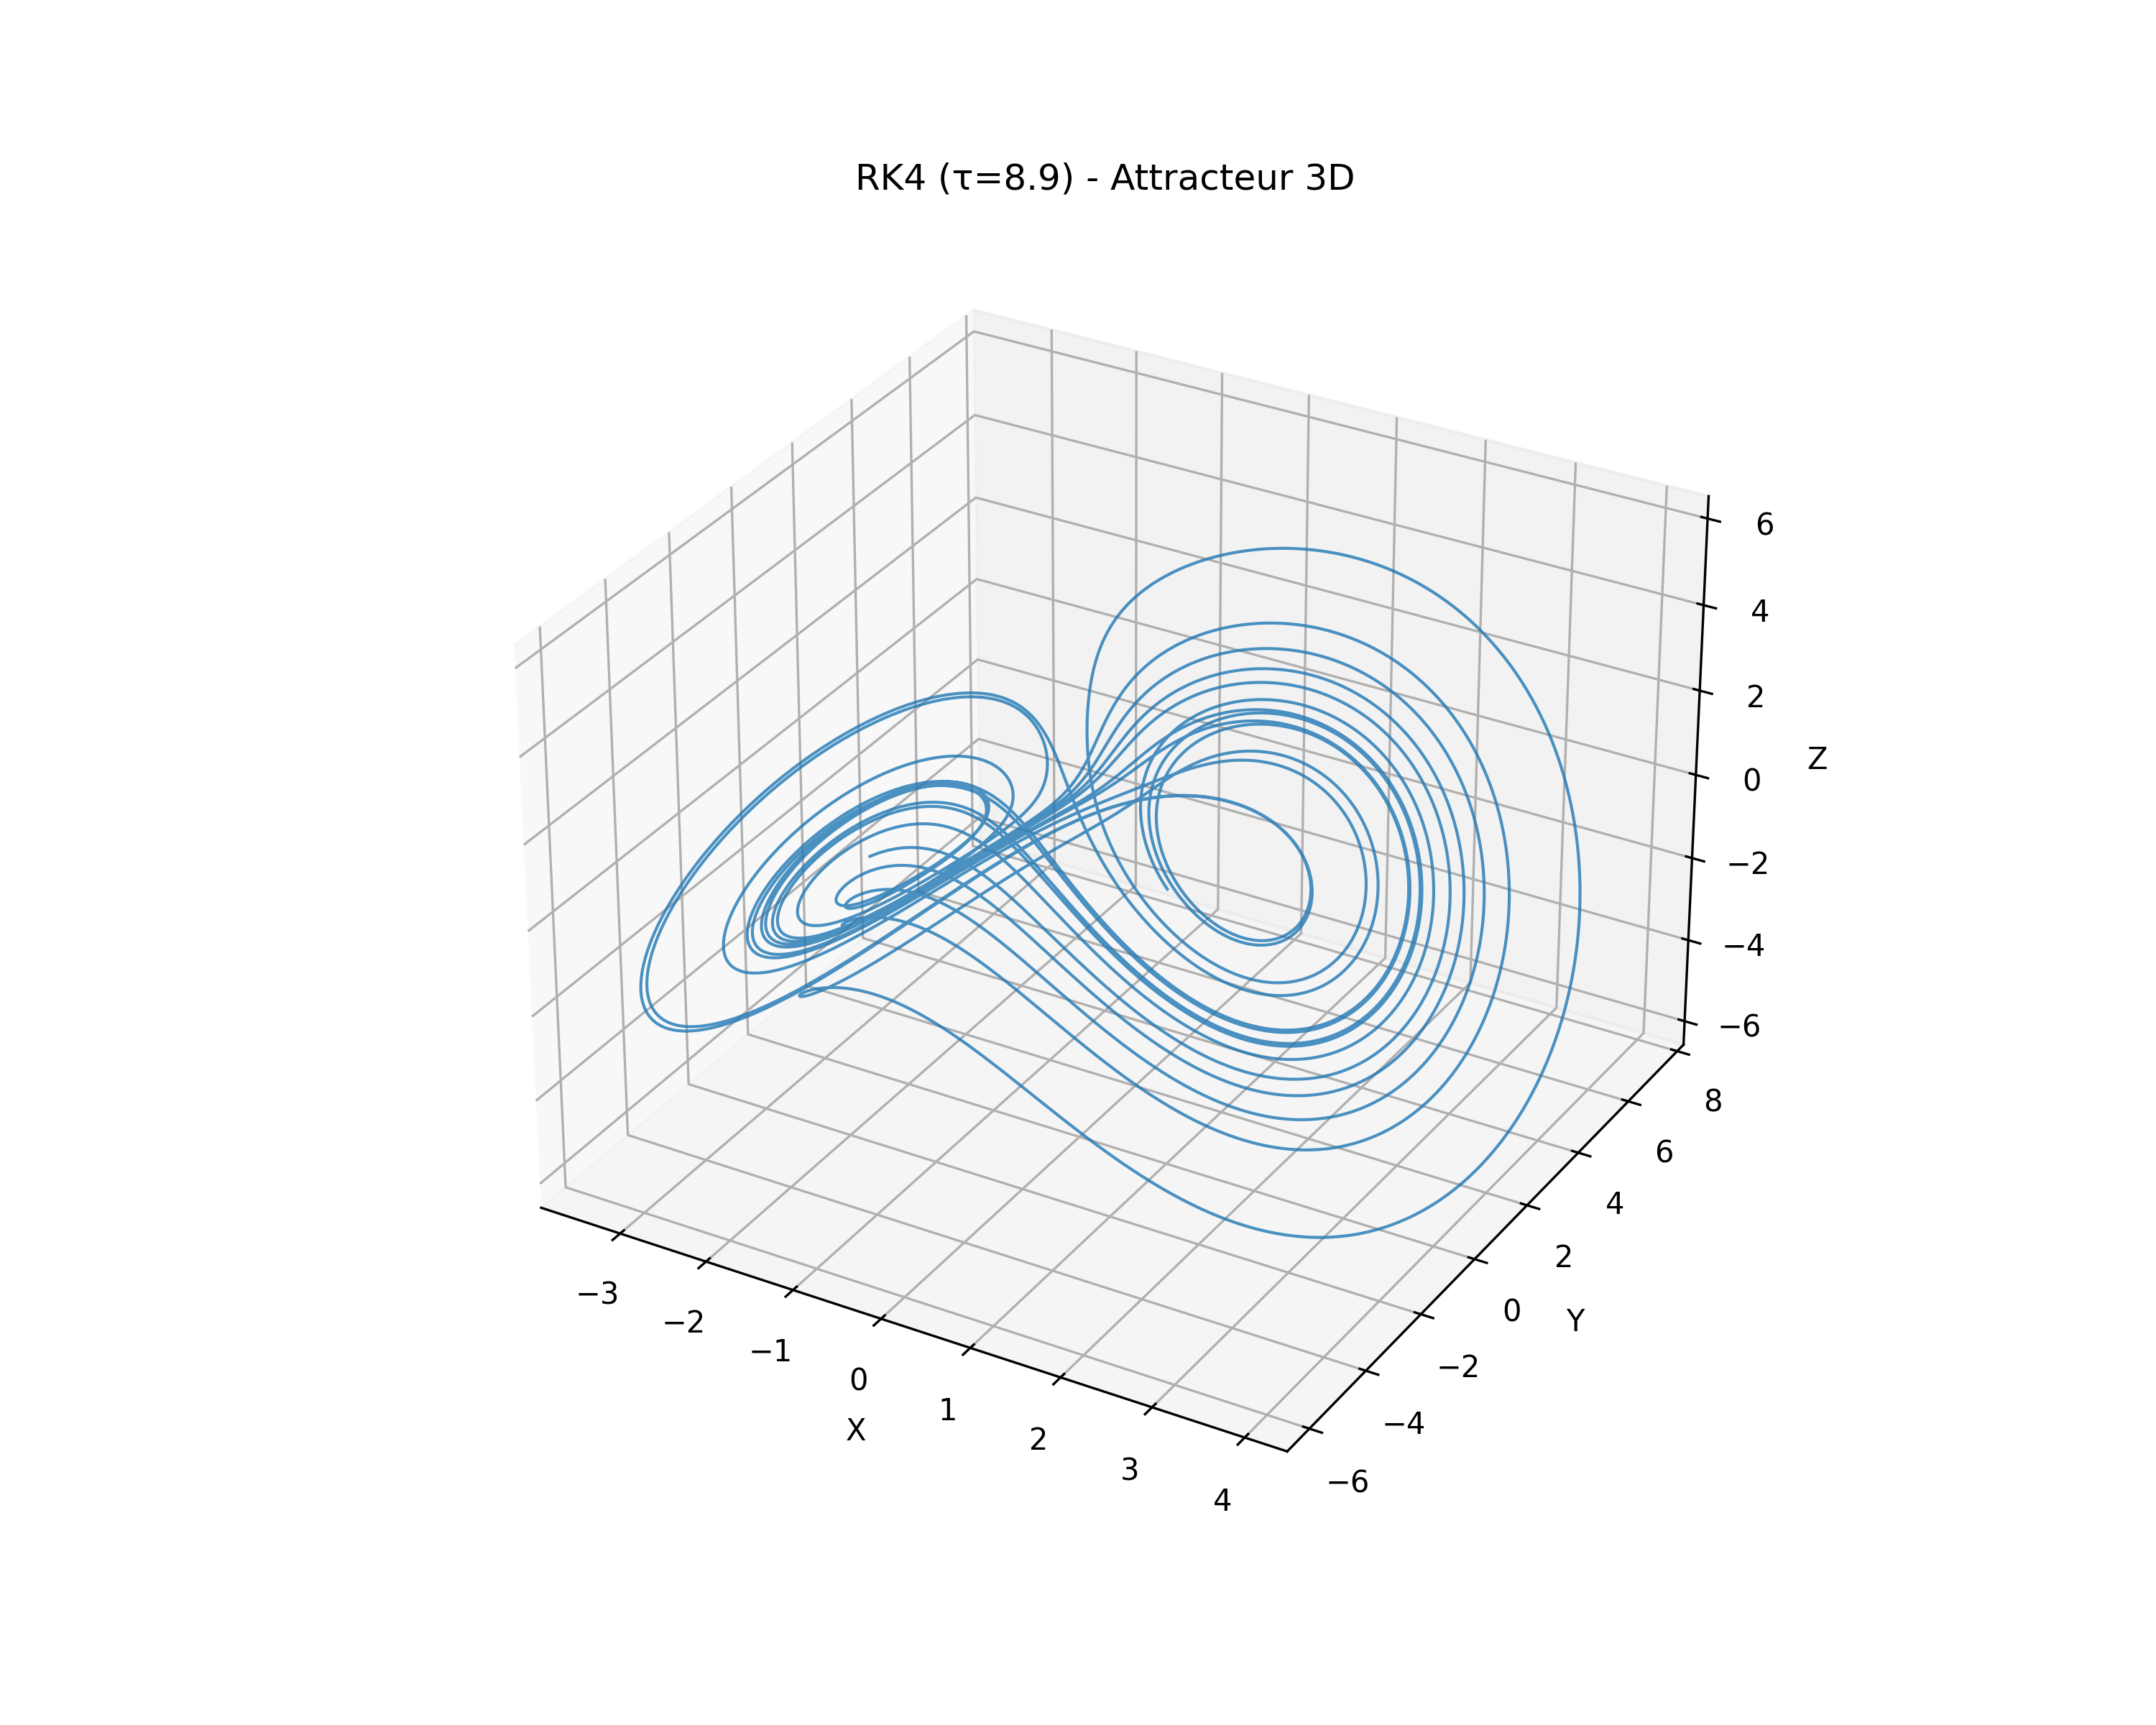
\includegraphics[width=\textwidth]{figures/rk4/rk4_tau8.9_3d}
        \caption{Trajectoire 3D : Structure intermédiaire entre l'attracteur chaotique et le point fixe}
    \end{subfigure}
    \begin{subfigure}[b]{0.4\textwidth}
        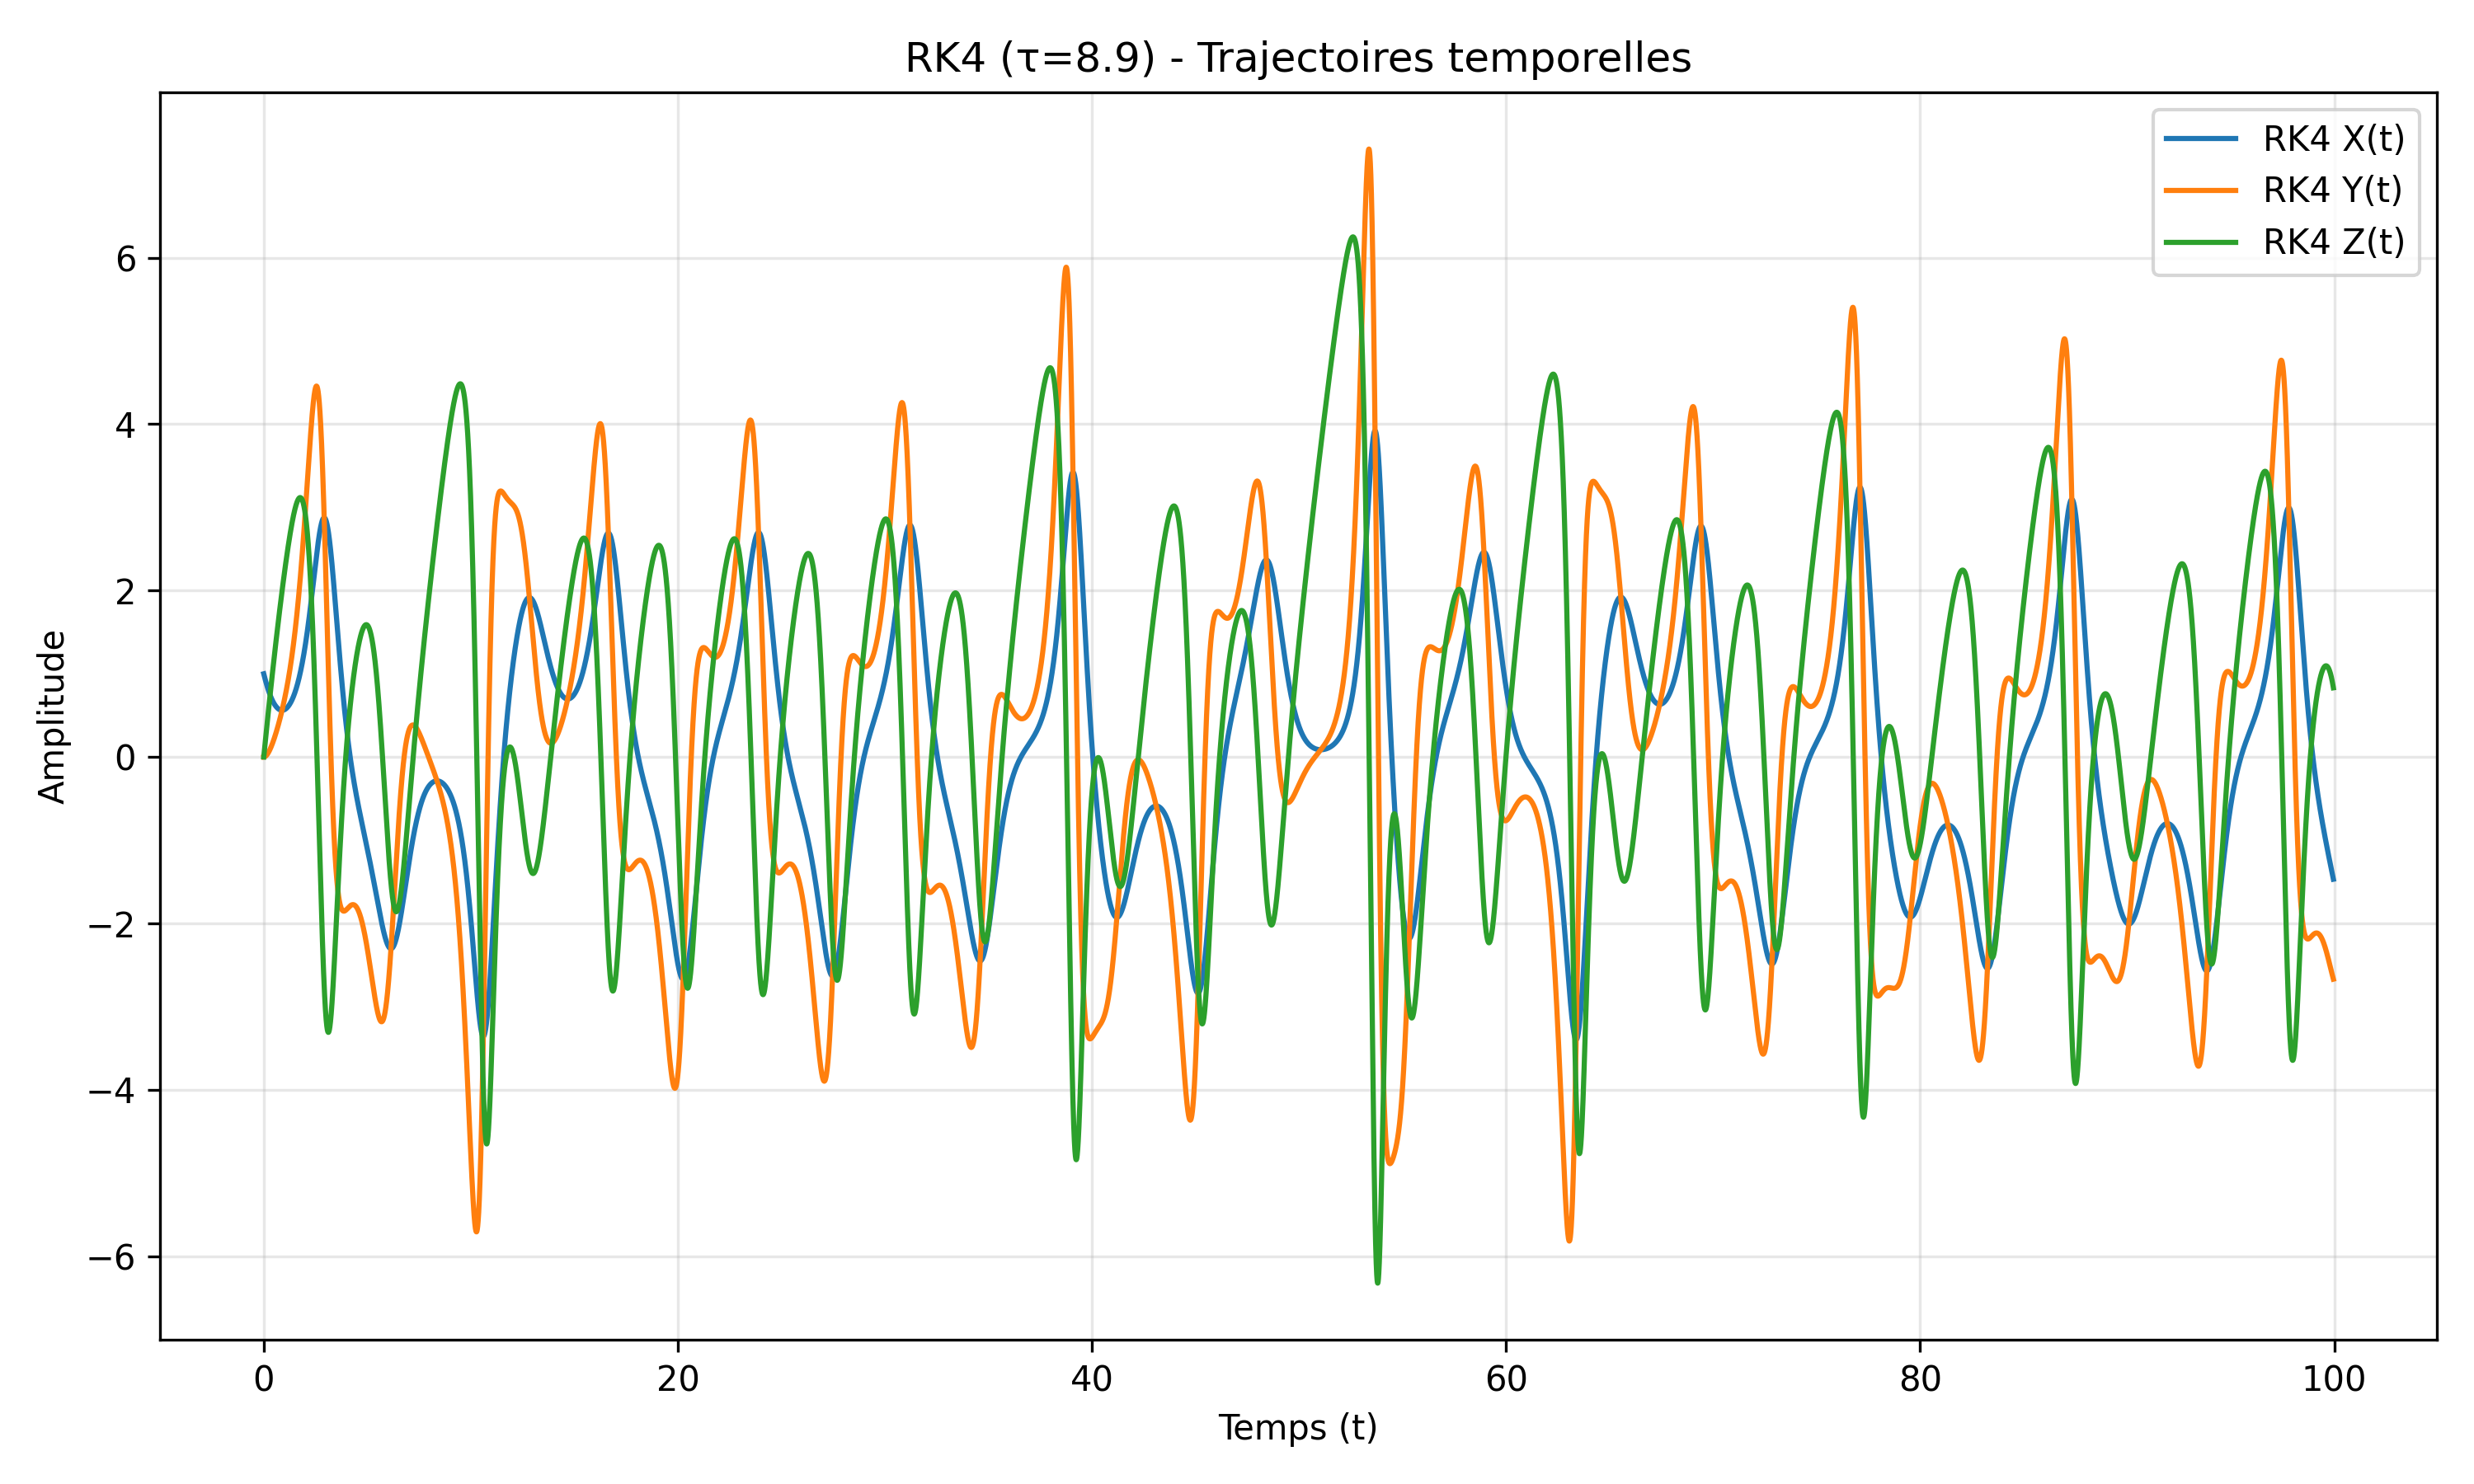
\includegraphics[width=\textwidth]{figures/rk4/rk4_tau8.9_time}
        \caption{Évolution temporelle : Oscillations avec une structure plus régulière mais avec dérive progressive}
    \end{subfigure}
    \begin{subfigure}[b]{0.3\textwidth}
        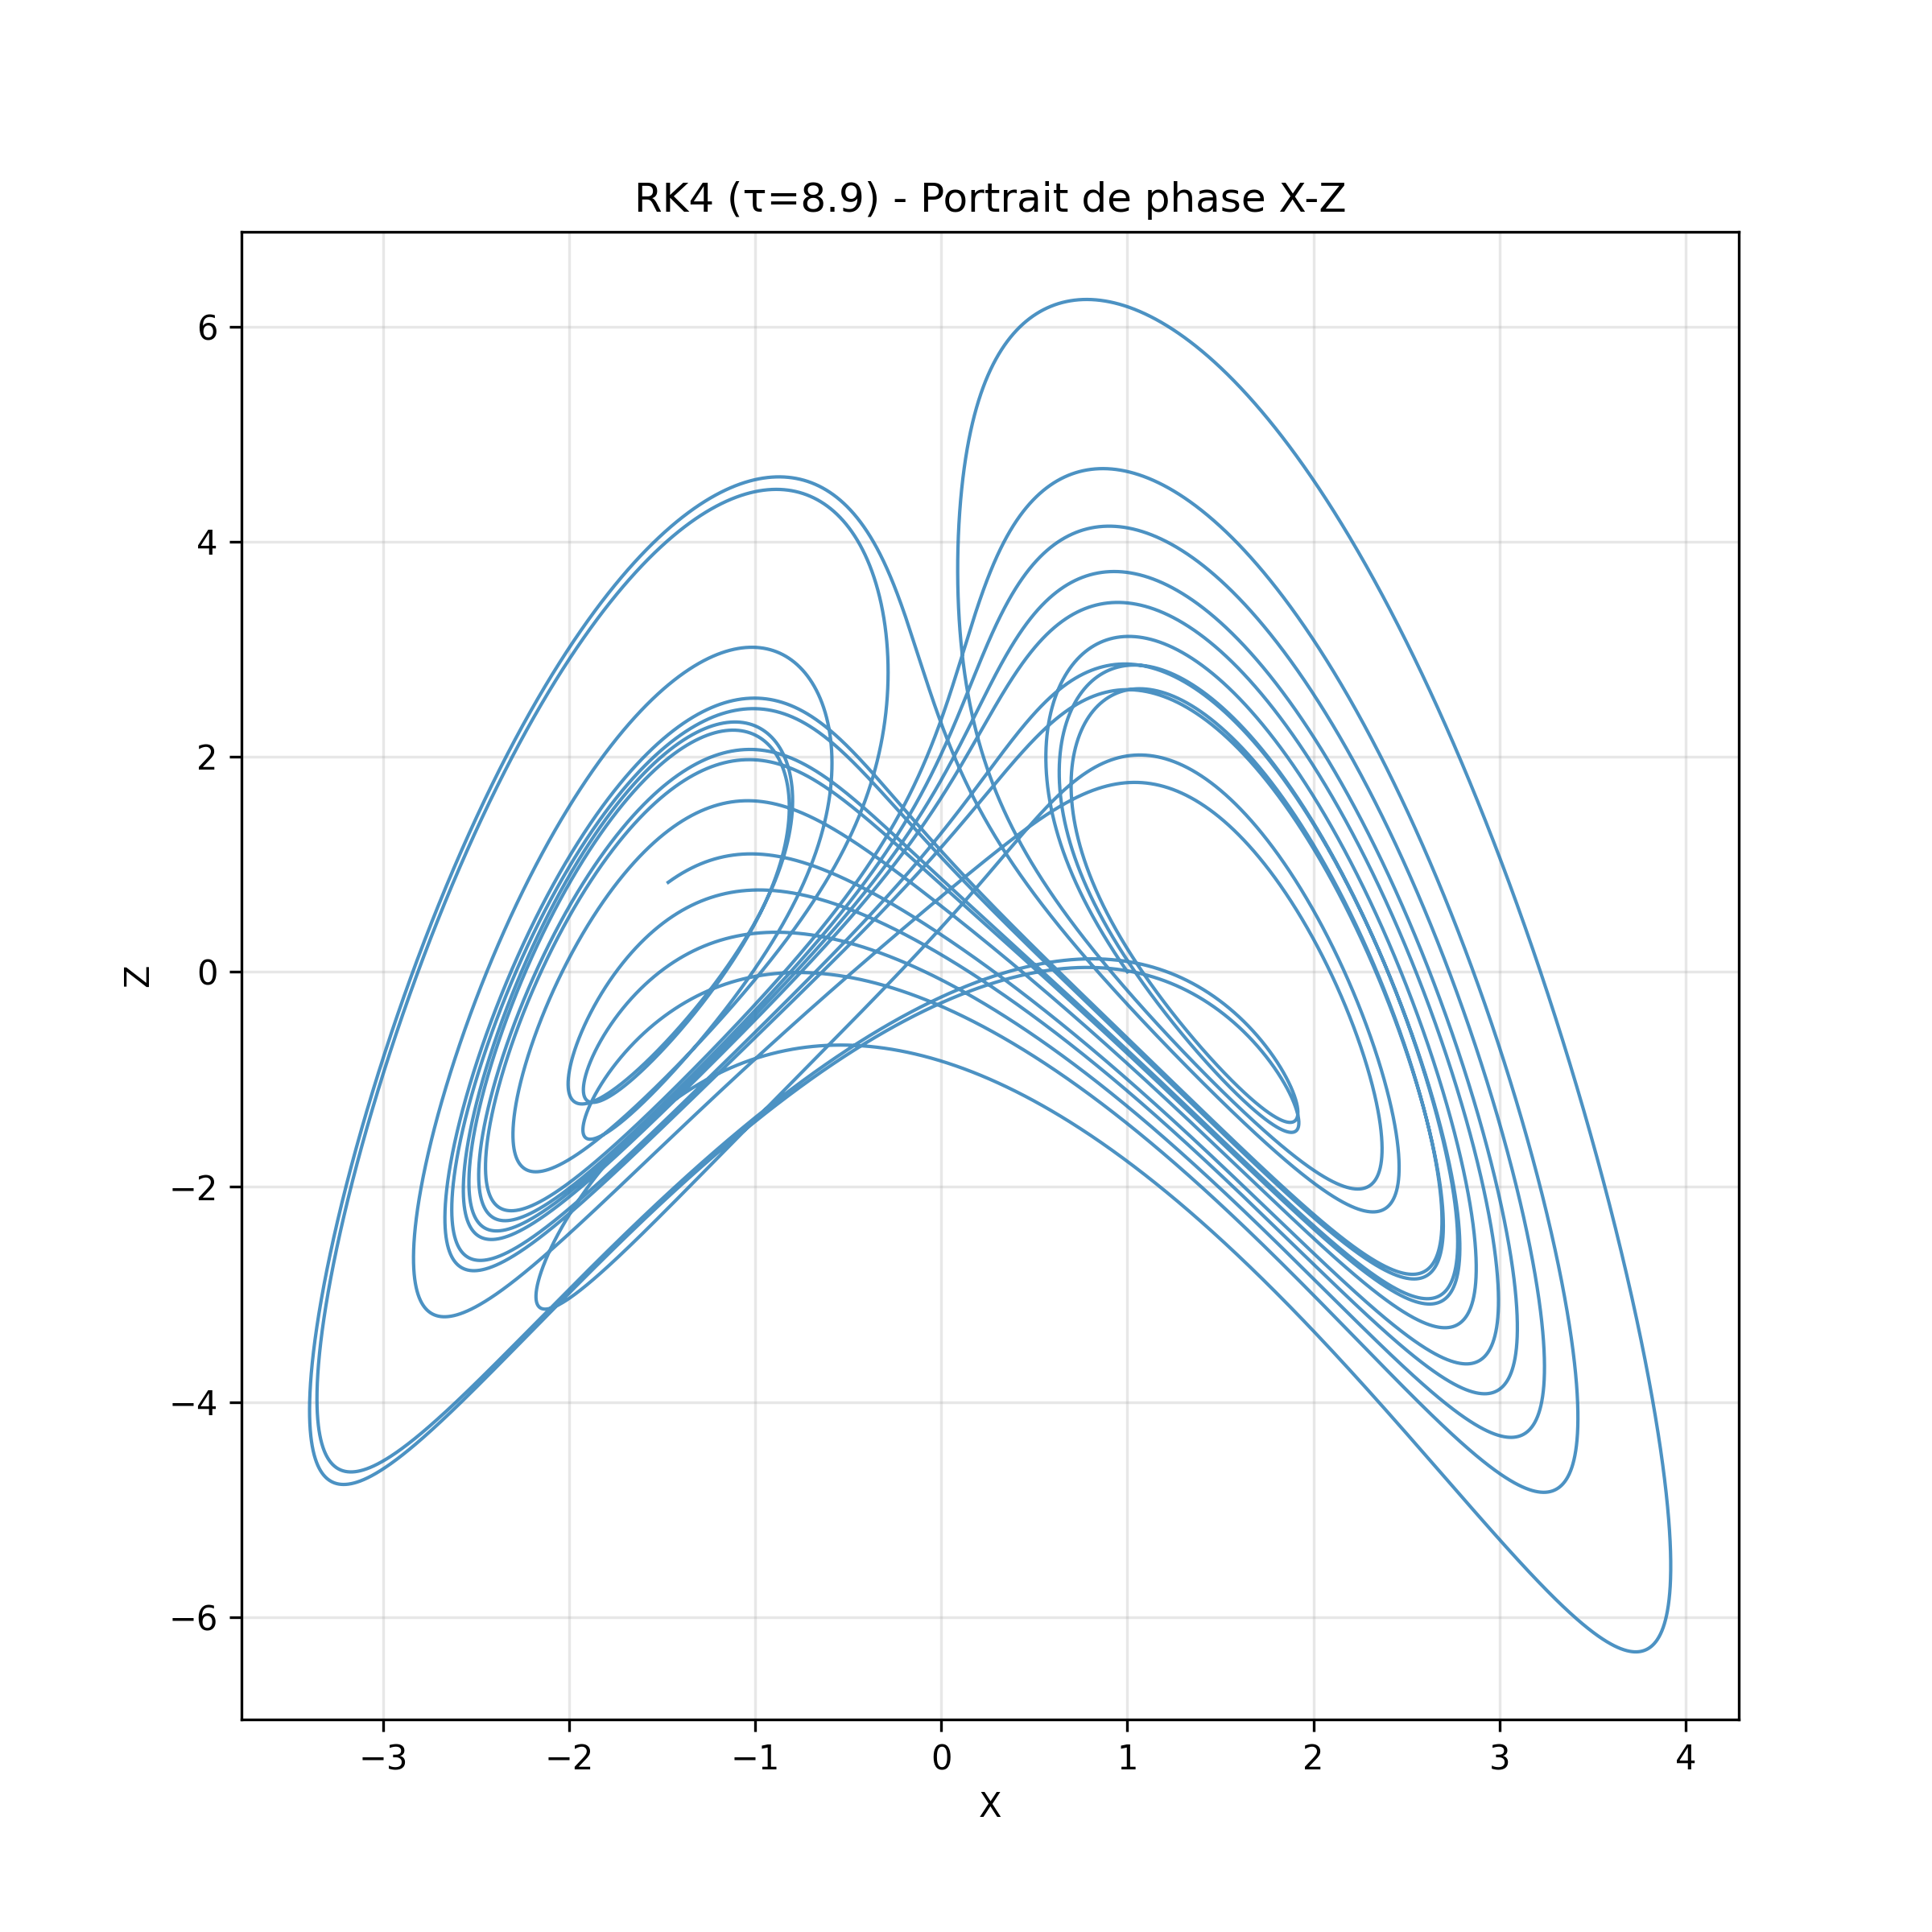
\includegraphics[width=\textwidth]{figures/rk4/rk4_tau8.9_phase}
        \caption{Portrait de phase : Trajectoire plus ordonnée mais non-périodique, formant un cycle limite déformé}
    \end{subfigure}
    \caption{Dynamique pour $\tau$ = 8.9 : comportement oscillatoire avec dérive}
    \label{fig:rk4_tau8.9}
\end{figure}

\subsection{Synthèse des résultats}
Les simulations numériques confirment parfaitement les comportements théoriques attendus pour chaque régime dynamique :

\begin{itemize}
    \item \textbf{État Non-Marcheur} ($\tau = 0.5$) : Convergence rapide vers l'origine, démontrant la stabilité du point fixe
    \item \textbf{Marche Régulière} ($\tau = 2.0$) : Établissement d'états stationnaires non nuls, caractéristiques du mouvement de marche
    \item \textbf{Marche Chaotique} ($\tau = 5.0$) : Comportement complexe avec attracteur étrange, typique du chaos
    \item \textbf{Oscillations avec Dérive} ($\tau = 8.9$) : Structure intermédiaire combinant oscillations et dérive progressive
\end{itemize}

\subsection{Limitations techniques}
La méthode RK4, bien que précise et stable, présente certaines limitations importantes :

\begin{enumerate}
    \item \textbf{Coût computationnel} : 4 évaluations de la fonction par pas de temps, rendant les simulations longues sur de grands intervalles
    \item \textbf{Stockage mémoire} : Nécessité de conserver les états intermédiaires, particulièrement problématique pour les systèmes de grande dimension
    \item \textbf{Parallélisation} : Impossible due à la dépendance séquentielle entre les pas de temps
\end{enumerate}

Ces limitations justifient l'exploration d'approches alternatives comme l'algorithme Parareal pour les simulations à grande échelle, particulièrement dans les régimes chaotiques où une haute précision est nécessaire.